\documentclass{article}

\usepackage[spanish]{babel}
\usepackage[utf8]{inputenc}
\usepackage{graphicx} % Required for the inclusion of images
\usepackage{amsmath} % Required for some math elements 
\usepackage{hyperref}
\usepackage{amsmath}
\usepackage{listings}
\usepackage{xcolor}
\usepackage{courier}
\usepackage[margin=1.2in]{geometry}
\usepackage{changepage}
\usepackage{titlesec}
\usepackage{wrapfig}
\usepackage{siunitx}

\definecolor{codegreen}{rgb}{0,0.6,0}
\definecolor{codegray}{rgb}{0.5,0.5,0.5}
\definecolor{codepurple}{rgb}{0.58,0,0.82}
\definecolor{backcolour}{rgb}{0.95,0.95,0.92}

\lstdefinestyle{mystyle}{
    backgroundcolor=\color{backcolour},   
    commentstyle=\color{codegreen},
    keywordstyle=\color{magenta},
    numberstyle=\tiny\color{codegray},
    stringstyle=\color{codepurple},
    basicstyle=\ttfamily\footnotesize,
    breakatwhitespace=false,         
    captionpos=b,                    
    keepspaces=true,                 
    numbers=left,                    
    numbersep=5pt,                  
    showspaces=false,                
    showstringspaces=false,
    showtabs=false,                  
    tabsize=2
}
\lstset{language=Python, 
        basicstyle=\ttfamily\small, 
        keywordstyle=\color{keywords},
        commentstyle=\color{comments},
        stringstyle=\color{red},
        showstringspaces=false,
        identifierstyle=\color{codepurple},
        keywords=[2]{pow},
        keywordstyle=[2]{\color{orange}},
}

\lstset{style=mystyle}

\setlength\parindent{0pt} % Removes all indentation from paragraphs

\renewcommand{\labelenumi}{\alph{enumi}.} % Make numbering in the enumerate environment by letter rather than number (e.g. section 6)

%\usepackage{times} % Uncomment to use the Times New Roman font

%----------------------------------------------------------------------------------------
%	DOCUMENT INFORMATION
%----------------------------------------------------------------------------------------

\title{\textbf{Estudio de la oscilación \\ de un péndulo simple}} % Title

\author{Víctor Mira Ramírez} % Author name

\date{\today} % Date for the report

\begin{document}

\maketitle % Insert the title, author and date

\begin{center}
\begin{tabular}{l r}

Profesora: & María Reyes Calvo Urbina \\
Lugar: & Universidad de Alicante
\end{tabular}
\end{center}

\tableofcontents

% If you wish to include an abstract, uncomment the lines below
% \begin{abstract}
% Abstract text
% \end{abstract}

%----------------------------------------------------------------------------------------
%	SECTION 1
%----------------------------------------------------------------------------------------

\section{Introducción y Datos}
\subsection{Abstract}
Este experimento estudia el movimiento de un péndulo simple: el ángulo que describe, su velocidad angular, la tensión en la cuerda y el periodo. Analizaremos el caso con rozamiento y el caso sin él. La práctica incluye gráficas realizadas con códigos en python que representan el comportamiento del péndulo para varios ángulos iniciales y en diferentes intervalos de tiempo.

\subsection{Datos Empíricos}
\begin{tabular}{ll}
Masa del péndulo & 1\si{kg}\\
Longitud de la cuerda& 1\si{m}\\
\end{tabular}



\subsection{Diagramas y formulaciones matemáticas}

El siguiente diagrama muestra un péndulo simple y las fuerzas que actúan sobre él. Podemos descomponer el peso en una componente radial ($P_{r} = m g \cos(\theta) $) y en una componente tangencial ($P_{t} = m g \sin(\theta) $)

\begin{figure}[h]
\centering
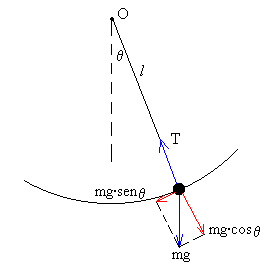
\includegraphics[width=.6\textwidth]{diagrama.png}
\end{figure}

Estudiamos el caso tanto en sentido radial, $ T - m g \cos(\theta) = m a_{c} = m l \omega^{2}$, donde $a_{c}$ es la aceleración centrípeta ($\frac{v^{2}}{r}$), quedándonos la ecuación para el periodo: \[ \boxed{T = m g \cos(\theta) + m l \omega^{2}}\] y el caso en sentido tangencial, $ -m g \sin(\theta) = m a_{t} = m l \alpha = m l \frac{d^{2}\theta}{dt^{2}}$, donde $a_{t}$ es la aceleración tangencial ($\frac{dv}{dt}$), quedándonos la ecuación para el ángulo: \[\boxed{\frac{d^{2}\theta}{dt^{2}} + \frac{g}{l} \sin(\theta) = 0}\] \\\\ Con esta ecuación diferencial, conseguimos el ángulo en función al tiempo, $ \omega(t)$, a partir de la cual podemos averiguar la velocidad angular, $\omega(t) = \frac{d\theta}{dt}$ y la aceleración angular $\alpha(t) = \frac{d^{2}\theta}{dt^{2}}$

Resolver esta ecuación diferencial es algo complicado, pero existe un método rápido para obtener soluciones para ángulos pequeños.

\subsubsection{Ángulos Pequeños}
La ecuación $\frac{d^{2}\theta}{dt^{2}} + \frac{g}{l} \sin(\theta) = 0$ puede simplificarse si, considerando ángulos pequeños, $\sin(\theta) = 0$, obteniendo la fórmula $\frac{d^{2}\theta}{dt^{2}} + \frac{g}{l} \theta) = 0$, que tiene una solución exacta, \[ \boxed{\theta = \theta_0 \cos(\gamma t)\ \ \ \ \ \ \ \theta_0 = \theta (t = 0)}\] donde $\gamma$ es la frecuencia angular, $\gamma^{2} = \frac{g}{l} \ \ \longrightarrow\ \ \ \gamma = \sqrt{\frac{g}{l}}$\\\\
y como $\omega = \frac{d\theta}{dt}$: \[\boxed{\omega = \theta_0 \gamma \left(-\sin(\gamma t)\right)} \]

\subsubsection{Solución Numérica}
Discretizando el tiempo y usando el método de Euler para pasos de $\Delta t$ pequeños, \\
$\omega = \frac{d\theta}{dt}\ \ \longrightarrow\ \ \ \frac{d^{2}\theta}{dt^{2}} + \frac{g}{l}\sin(\theta) = 0\ \ \longrightarrow\ \ \ \frac{d\omega}{dt} + \frac{g}{l}\sin(\theta) = 0\ \ \longrightarrow\ \ \ \Delta\omega = \left[ \frac{-g}{l}\sin(\theta)\right] \Delta t$ \\
y por tanto, obtenemos para la velocidad angular la ecuación: \[ \boxed{\omega_{i+1} = \omega_{i} - \left(\frac{g}{l}\sin(\theta_{i})\right)\Delta t}\] 
\\ y como $\omega = \frac{d\theta}{dt}\ \ \rightarrow\ \ \Delta \theta = \omega \Delta t$, obtenemos para el ángulo la ecuación: \[ \boxed{\theta_{i+1} = \theta_{i} + \omega_{i} \Delta t}\]

\subsubsection{Energías}
Trivialmente sabemos que la Energía Mecánica será la suma de la Energía Potencial y de la Energía Cinética. En el caso sin rozamiento, habrá una conservación de la Energía Mecánica, ya que no existirá ninguna energía disipatoria que la reduzca. Ese es el caso con rozamiento, donde el rozamiento irá poco a poco reduciendo nuestra energía mecánica total hasta llegar al punto donde no oscilará.
\paragraph{Energía Potencial}\mbox{}\\\\
Sabiendo que la fórmula de la Energía Potencial es $E_{p} = -m g h$ y que la altura del péndulo en cada momento viene dada por $\cos(\theta)l$, obtenemos para la Energía Potencial de nuestro péndulo la ecuación: \\\[ \boxed{E_{p} = -m g l \cos(\theta)}\]
\paragraph{Energía Cinética}\mbox{}\\\\
Sabiendo que la fórmula de la Energía Cinética es $E_{c} = \frac{1}{2} m v^2$ y que la velocidad tangencial se relaciona con la angular con la fórmula $v = \omega r$, donde $r$ será la longitud de la cuerda del péndulo $l$, obtenemos para la Energía Cinética de nuestro péndulo la ecuación \\\[ \boxed{E_{c} = \frac{1}{2} m \omega^{2} l^{2}}\]

\subsubsection{Péndulo con Fricción}
La fuerza de rozamiento viene definida por la ecuación $F_{r} = -k \omega$, que debemos agregar a nuestra ecuación diferencial inicial, quedándonos la nueva ecuación diferencial: \[ -m g \sin(\theta) - k \omega = m l \alpha = m l \frac{d^2\theta}{dt^2} \] \[\boxed{\frac{d^{2}\theta}{dt^{2}} + \frac{g}{l} \sin(\theta) - \frac{k}{m l} \frac{d\theta}{dt} = 0}\]
Simplemente hemos añadido el término $- \frac{k}{m l} \frac{d\theta}{dt} = 0$ a nuestra ecuación diferencial.\\ \\
Actualizando nuestra solución numérica tenemos las siguientes ecuaciones para el caso con rozamiento:
\[ \boxed{\omega_{i+1} = \omega_{i} + \left[ \frac{-g}{l} \sin(\theta_{i}) + \frac{k}{m l}\omega_{i} \right] \Delta t}\]
\[ \boxed{\theta_{i+1} = \theta_{i} + \omega_{i} \Delta t}\]
\\ \\
El siguiente diagrama representa el caso estudiado, donde T es la tensión y $F_{r}$ es la fuerza de rozamiento que hemos añadido.

\begin{figure}[h]
\centering
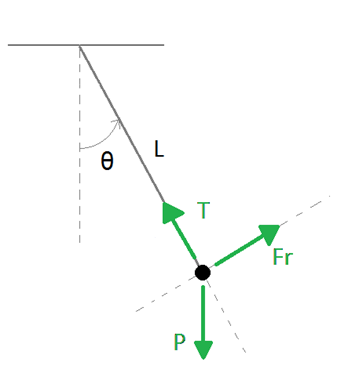
\includegraphics[width=.6\textwidth]{diagramarozamiento.png}
\end{figure}
%----------------------------------------------------------------------------------------
%	SECTION 4
%----------------------------------------------------------------------------------------
\section{Parte a) - Péndulo sin Fricción}
En esta sección estudiaremos las gráficas del movimiento del péndulo usando dos soluciones diferentes, una solución numérica de la ecuación diferencial, y otra para ángulos pequeños. Observaremos como para ángulos mayores a 15 grados, la solución numérica es la única que nos proporciona unos resultados más fiables.

\subsection{Cálculo del Ángulo, Velocidad Angular y la Tensión}
\subsubsection{Evolución del Ángulo en función del tiempo}
\begin{figure}[h]
\centering
\hspace*{-2.3cm}
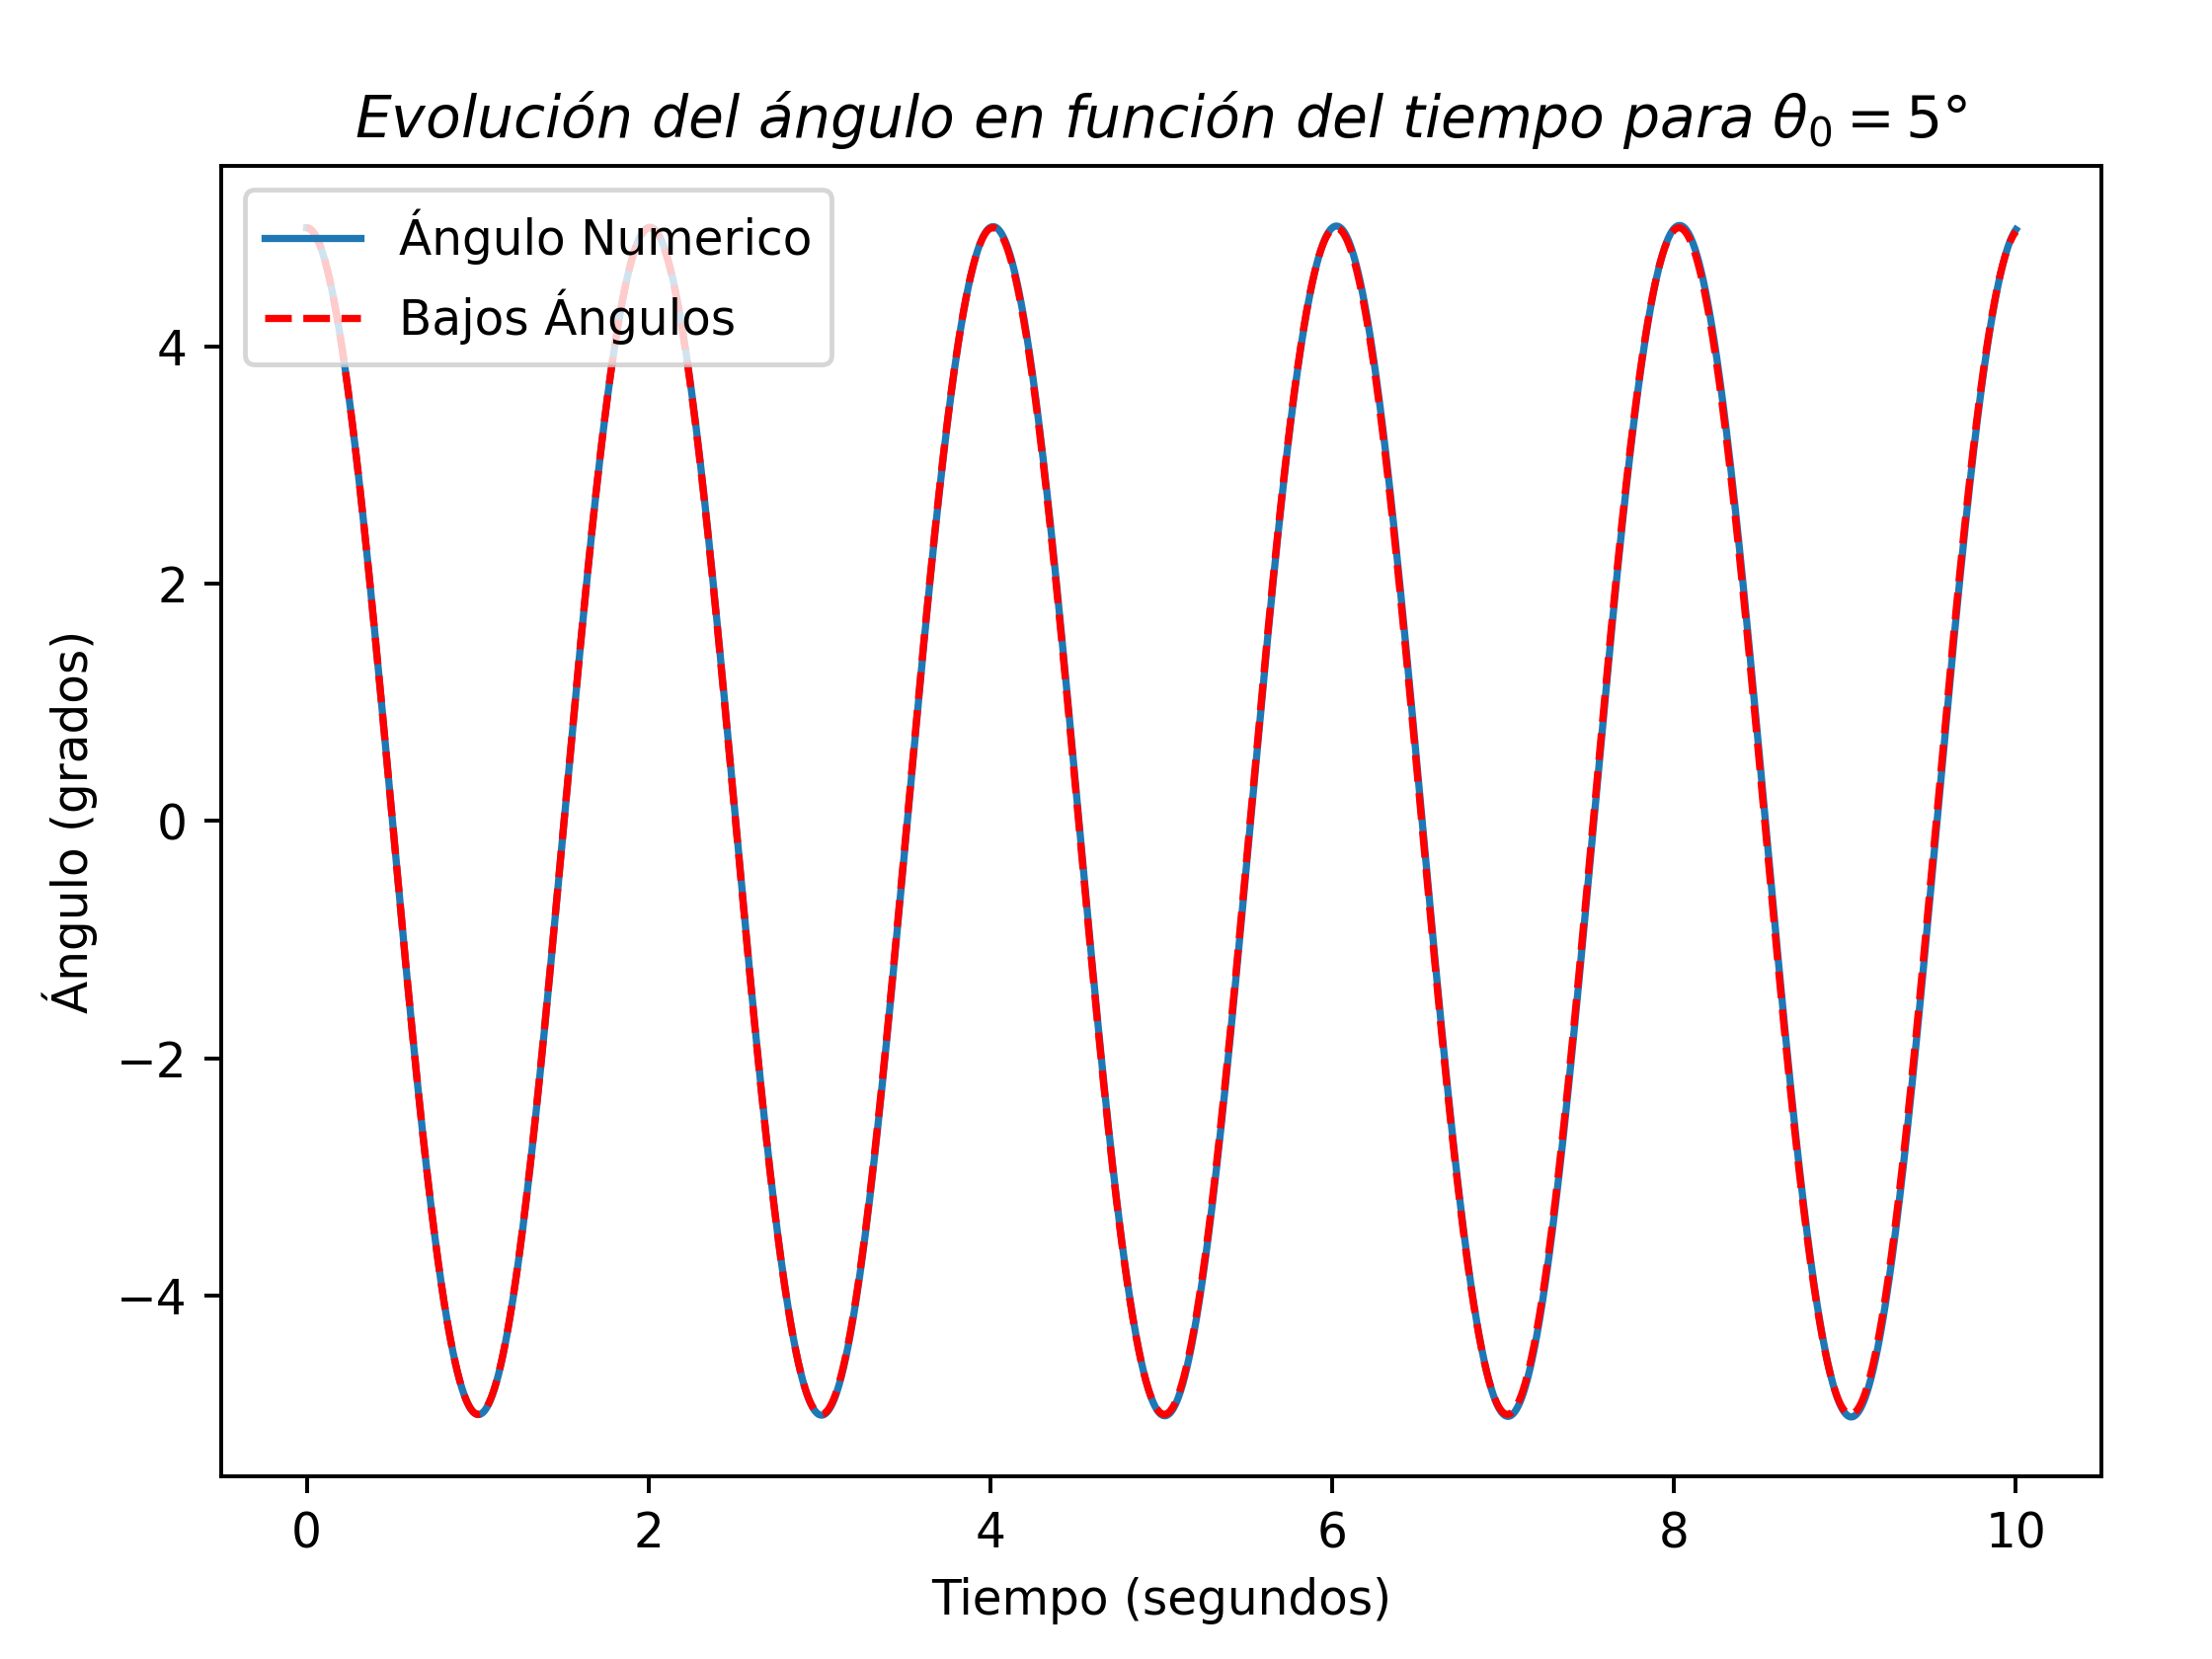
\includegraphics[width=.57\textwidth]{Fig1a.png}\hfill
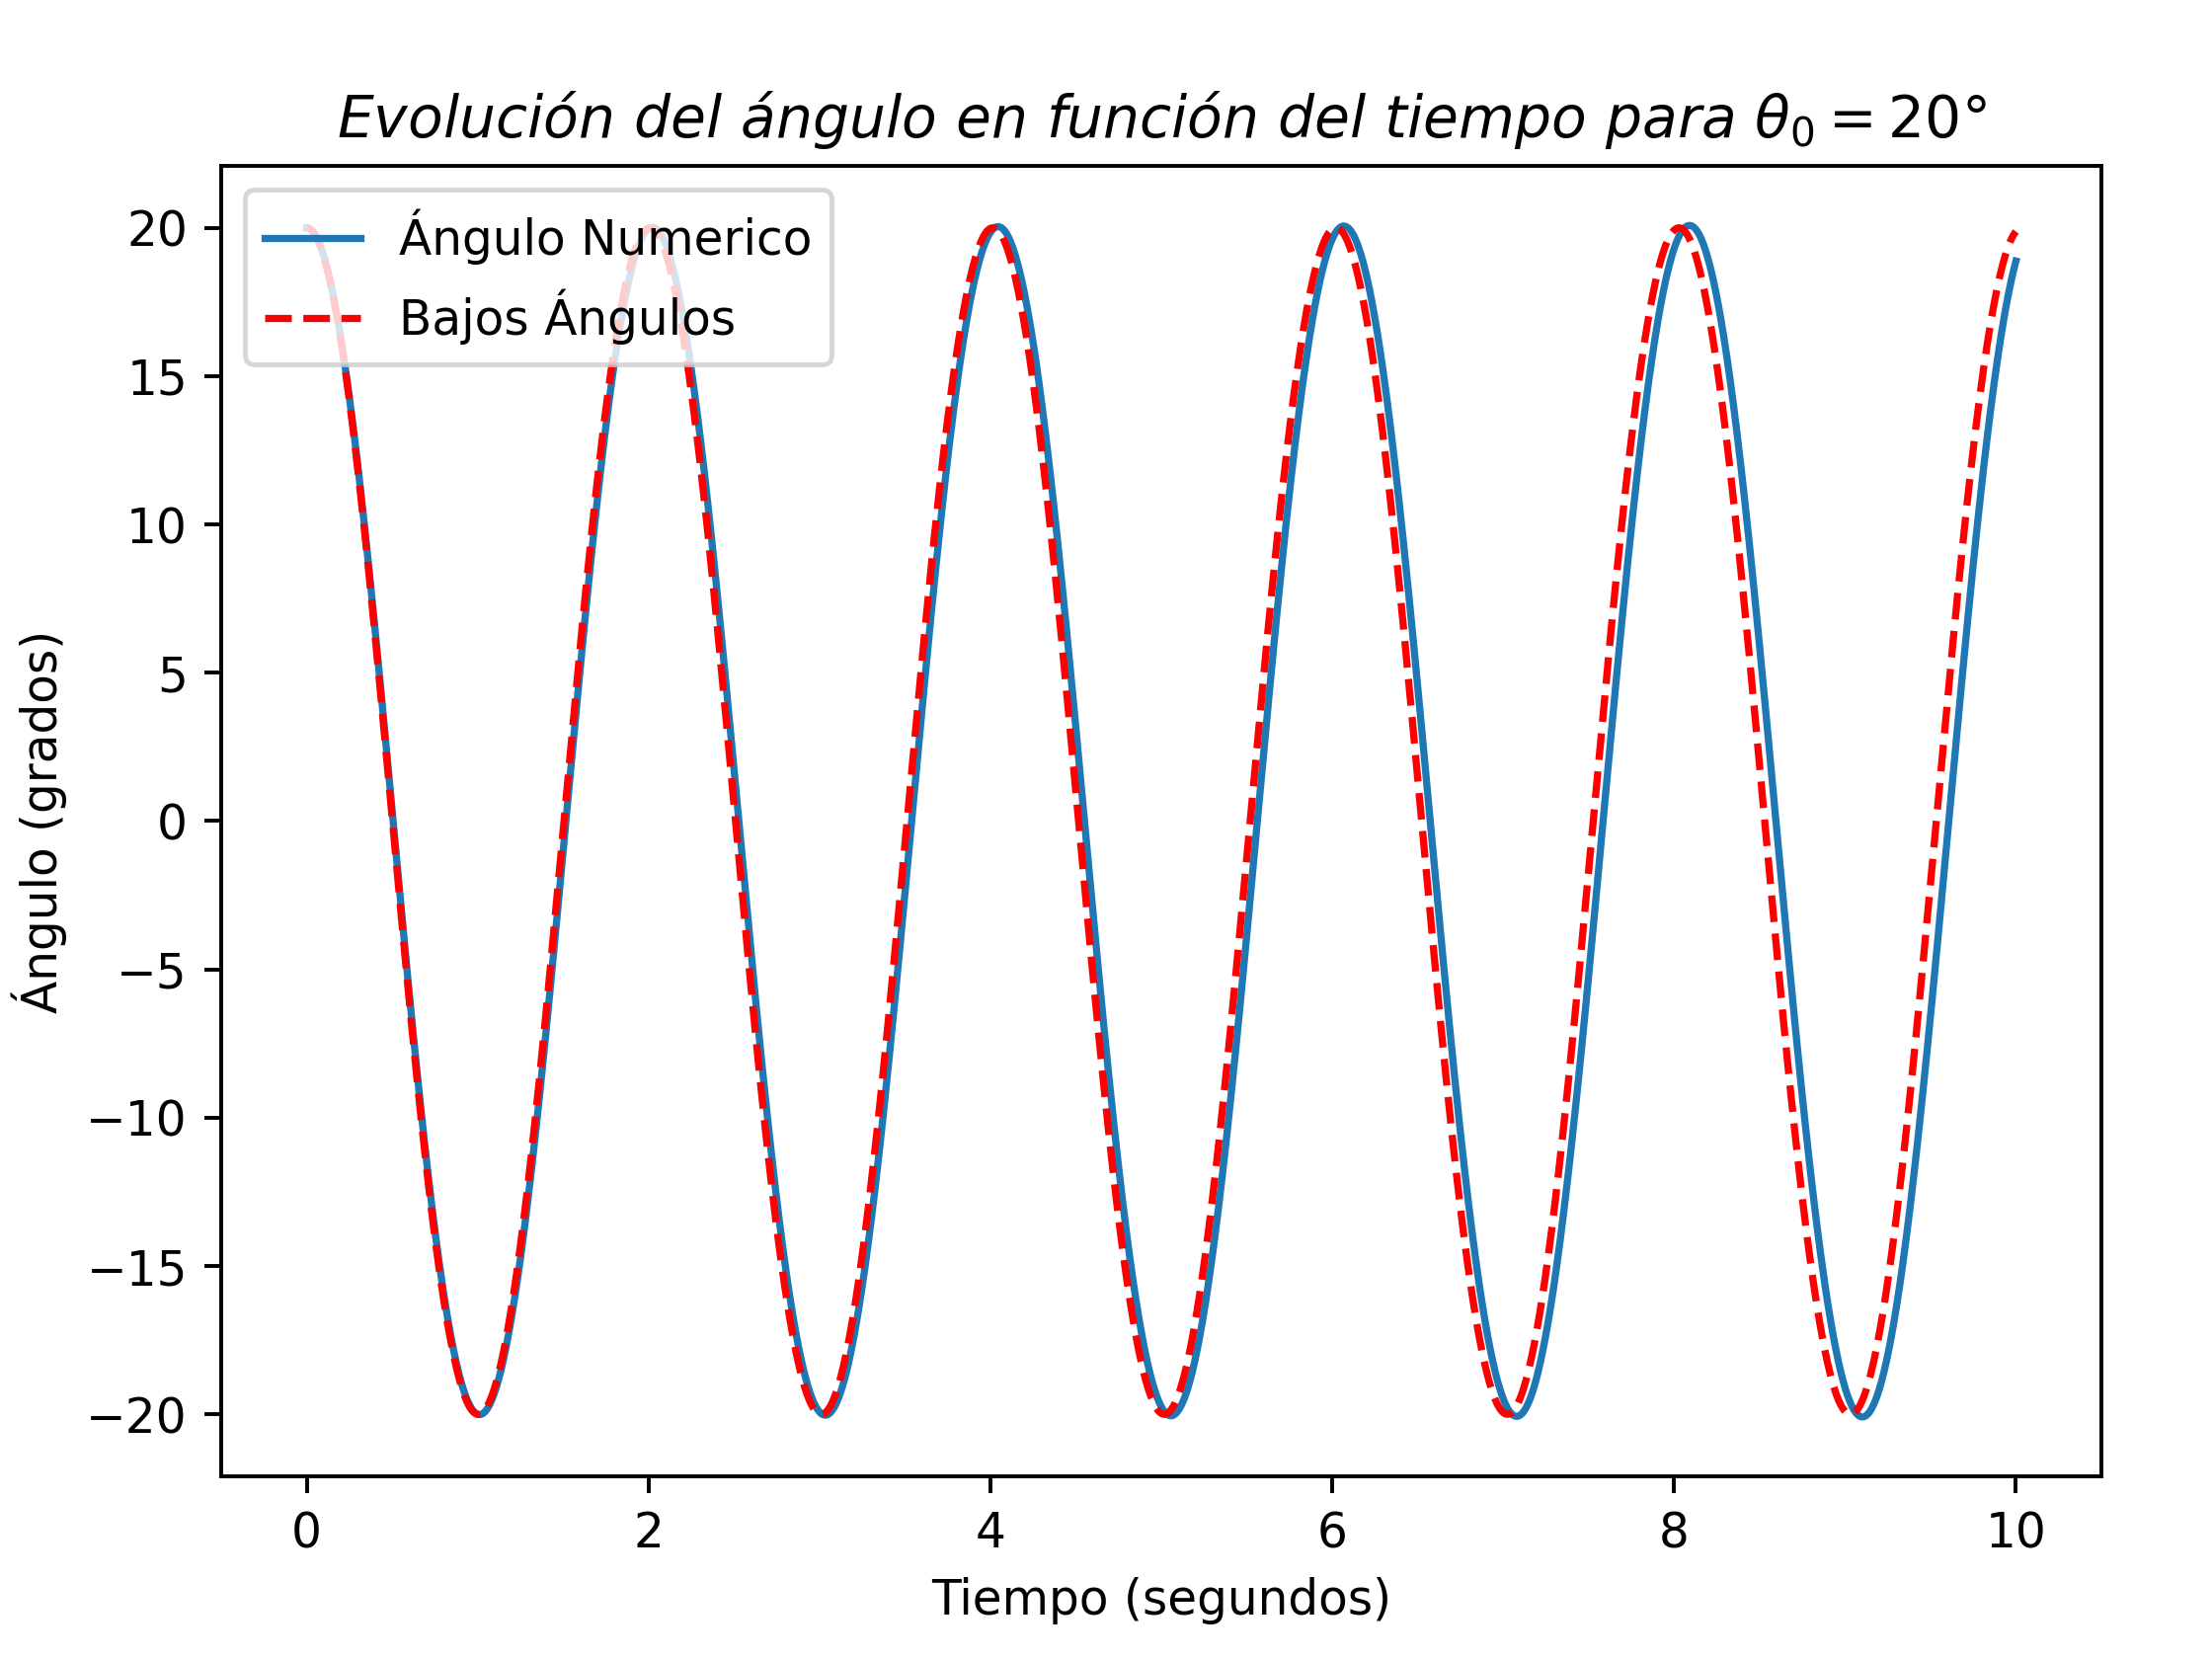
\includegraphics[width=.57\textwidth]{Fig2a.png}
\hspace*{-2.3cm}
\end{figure}
\begin{figure}[h]
\centering
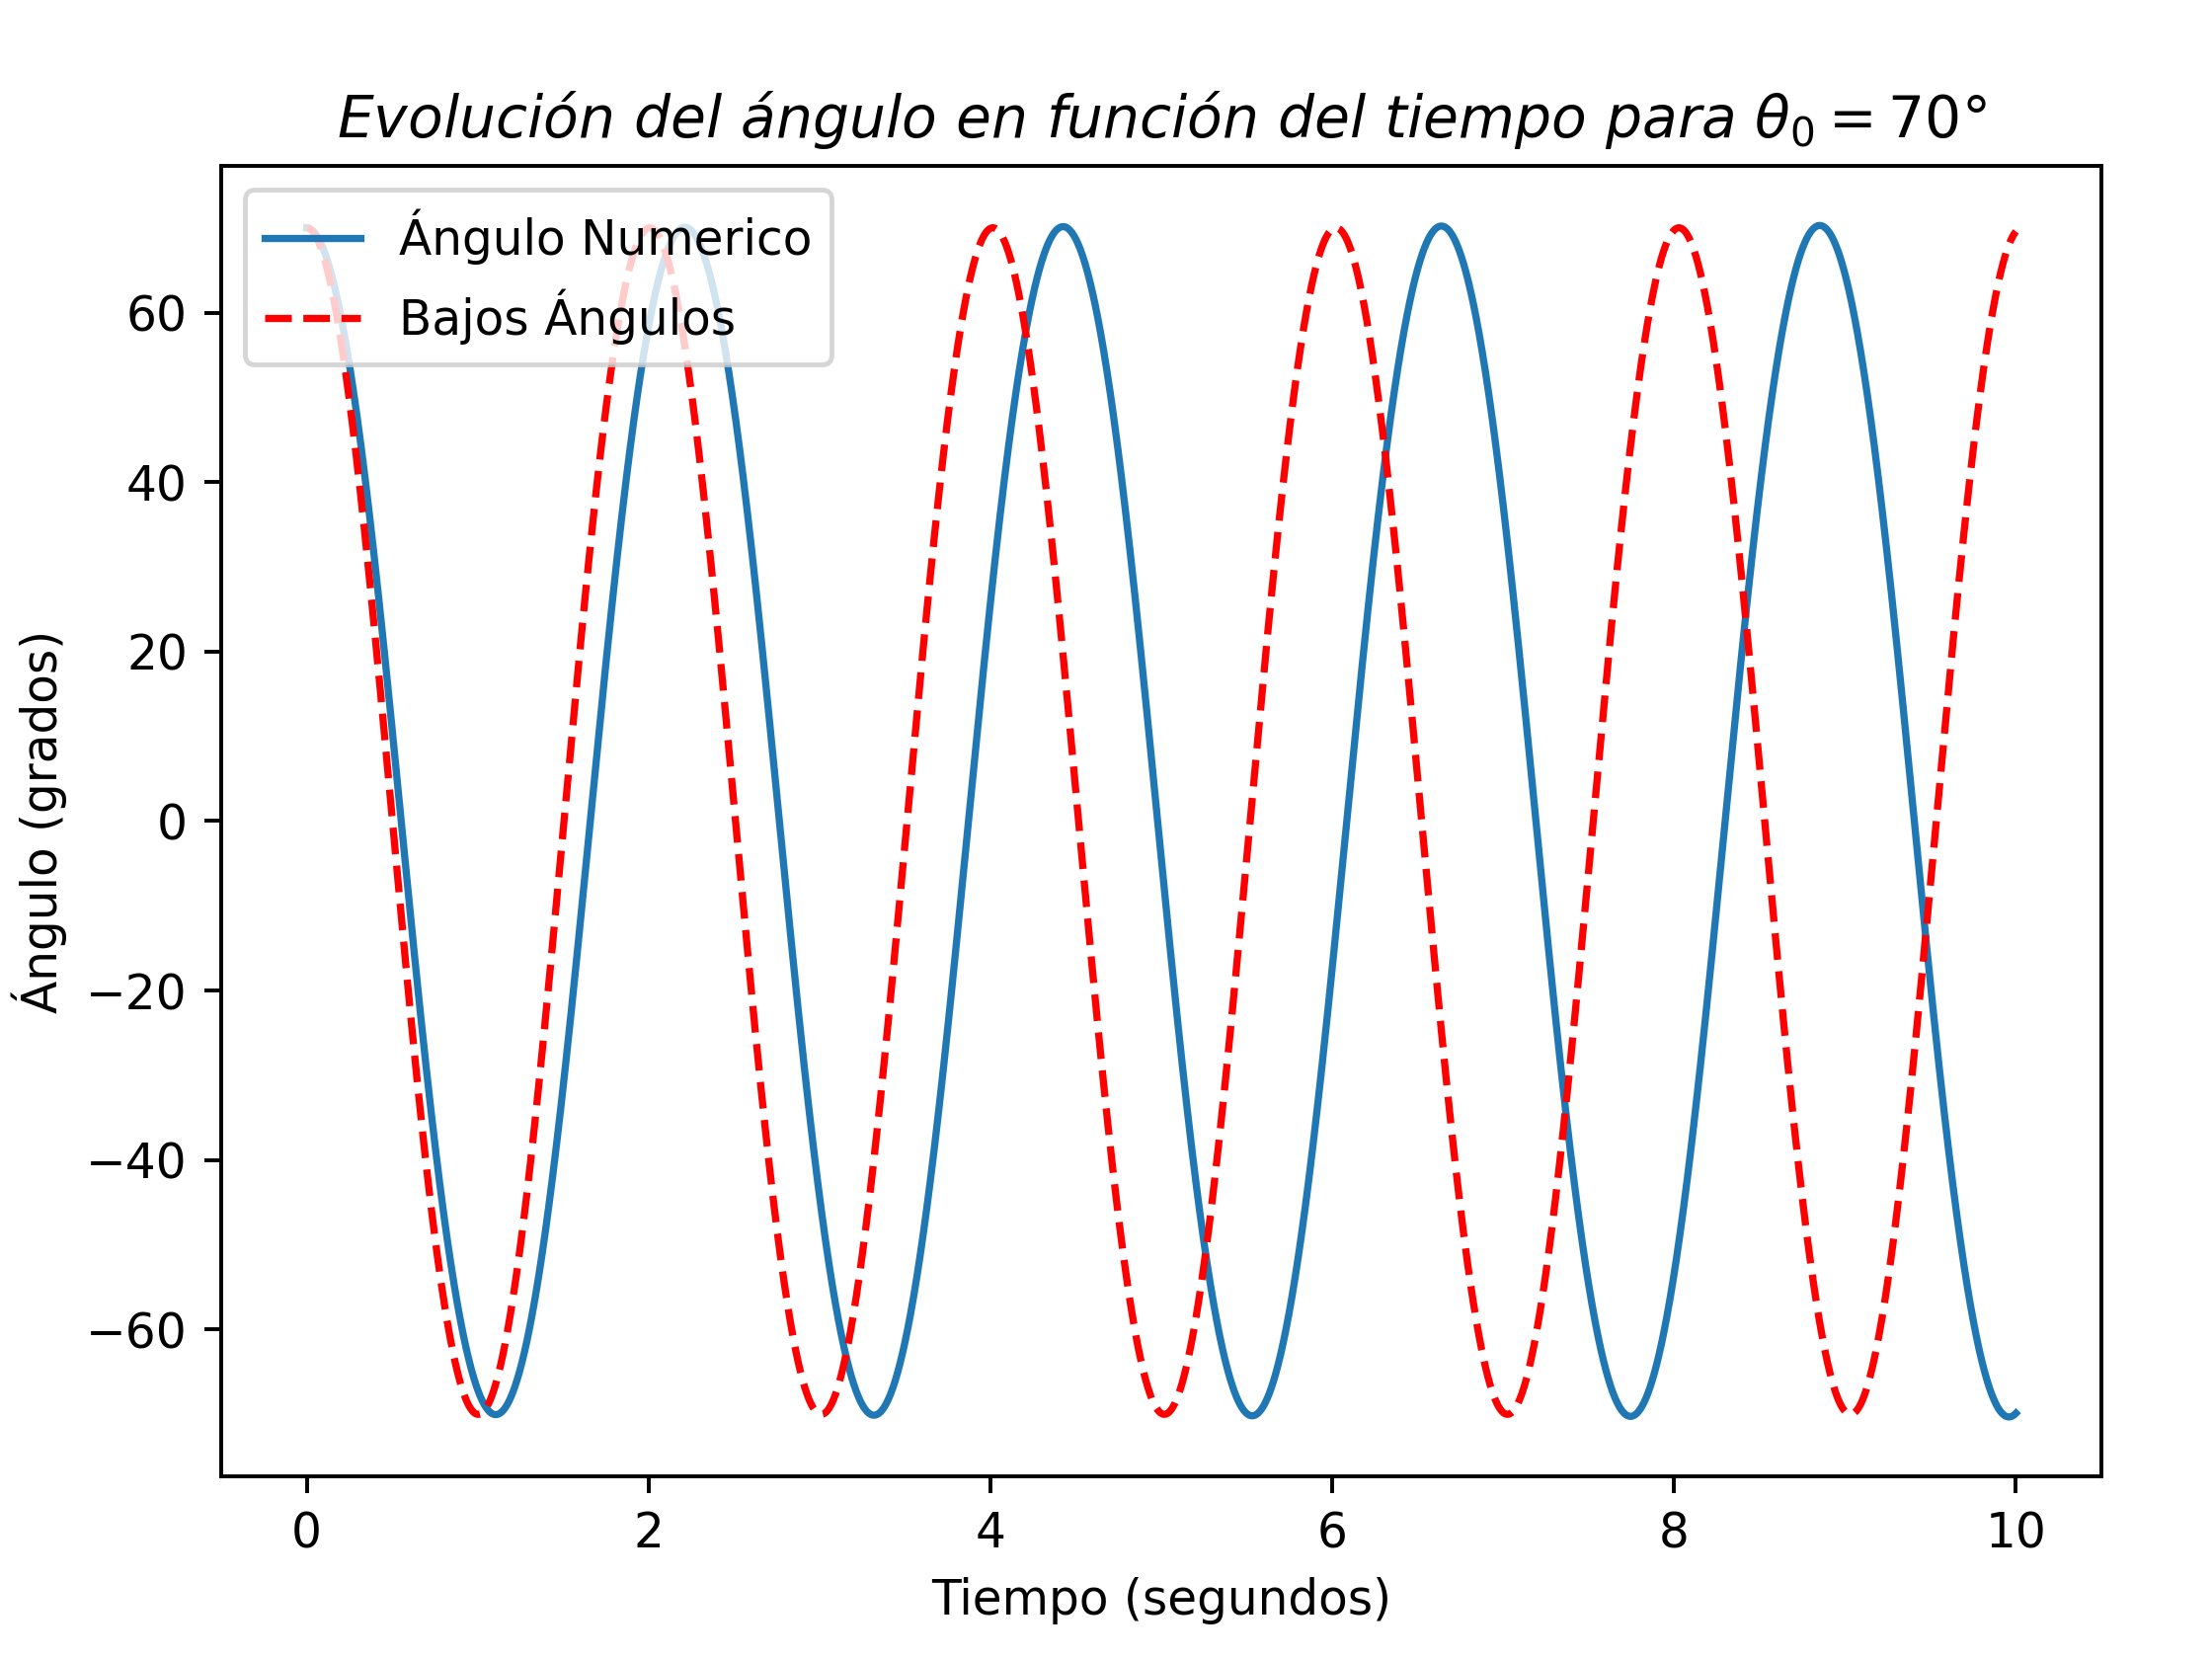
\includegraphics[width=.57\textwidth]{Fig3a.png}
\end{figure}

\hfill \break \\
Comentar como para 5$^\circ$ ambas soluciones coinciden casi a la perfección, para 20 $^\circ$ los métodos empiezan a distanciarse, y para 70$^\circ$ las soluciones se desfasan completamente en menos de 10 segundos. 

\pagebreak
\hfill \break \\
\hfill \break \\
\hfill \break \\

Código que calcula estas gráficas:
\begin{adjustwidth}{-8pt}{-8pt}
\lstinputlisting[language=Python, firstline=1, lastline=31]{1.py}
\end{adjustwidth}
%---------------------------------------------------------------
\pagebreak
\subsubsection{Evolución de la Velocidad Angular en función del tiempo}
\begin{figure}[h]
\centering
\hspace*{-2.3cm}
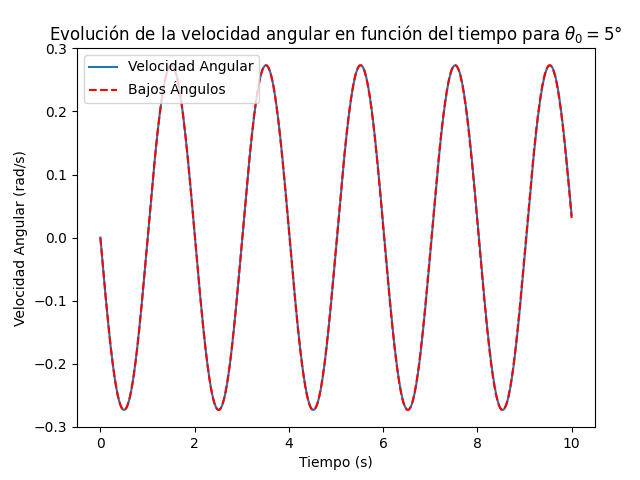
\includegraphics[width=.57\textwidth]{Fig1b.png}\hfill
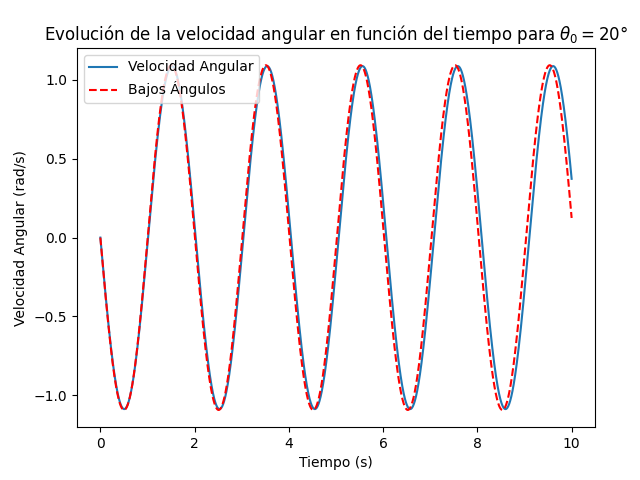
\includegraphics[width=.57\textwidth]{Fig2b.png}
\hspace*{-2.3cm}
\end{figure}
\begin{figure}[h]
\centering
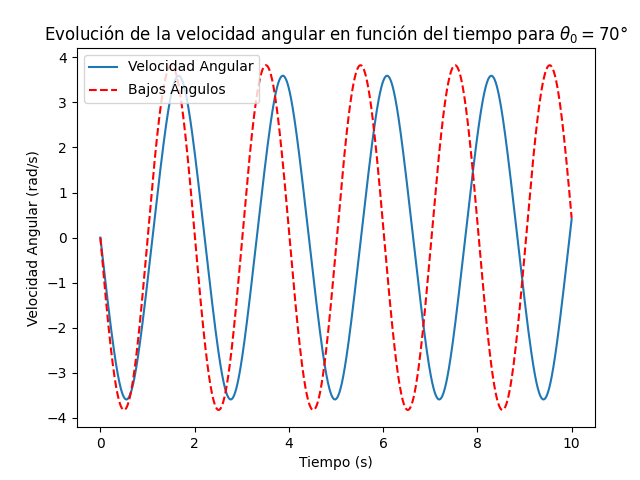
\includegraphics[width=.57\textwidth]{Fig3b.png}
\end{figure}

\hfill \break \\
Al igual que con la posición, la velocidad angular en la solución para ángulos pequeños se desfasa respecto de la solución numérica para ángulos superiores a unos 15$^\circ$

\pagebreak
\hfill \break \\
\hfill \break \\
\hfill \break \\

Código que calcula estas gráficas:
\begin{adjustwidth}{-38pt}{-38pt}
\lstinputlisting[language=Python, firstline=1, lastline=29]{2.py}
\end{adjustwidth}
%---------------------------------------------------------------
\pagebreak
\subsubsection{Evolución de la Tensión en función del tiempo}
\begin{figure}[h]
\centering
\hspace*{-2.3cm}
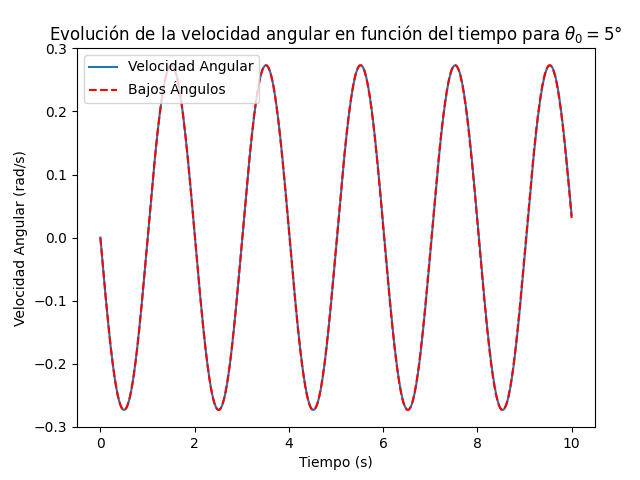
\includegraphics[width=.57\textwidth]{Fig1b.png}\hfill
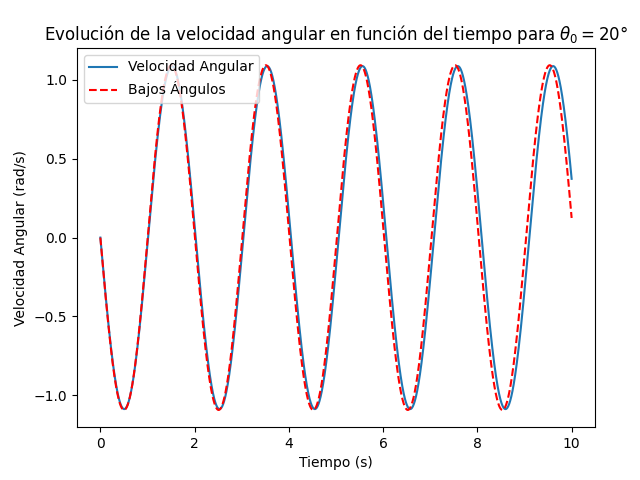
\includegraphics[width=.57\textwidth]{Fig2b.png}
\hspace*{-2.3cm}
\end{figure}
\begin{figure}[h]
\centering
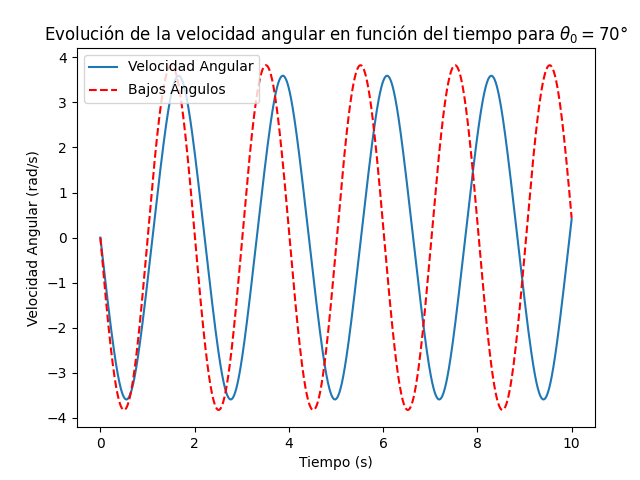
\includegraphics[width=.57\textwidth]{Fig3b.png}
\end{figure}

\hfill \break \\
De la misma forma que con la posición y la velocidad angular, las soluciones se desfasan en ángulos superiores a 15$^\circ$ rápidamente. 

\hfill \break \\
Concluimos que siempre que el ángulo sea pequeño y el tiempo en el que lo apliquemos sea razonable, la solución para ángulos pequeños es perfectamente válida, y equiparable a la numérica.

\pagebreak
Código que calcula estas gráficas:
\begin{adjustwidth}{-15pt}{-15pt}
\lstinputlisting[language=Python, firstline=1, lastline=26]{3.py}
\end{adjustwidth}

%----------------------------------------------------------------------------------------
%	SECTION 5
%----------------------------------------------------------------------------------------

\subsection{Cálculo del periodo de oscilación}

\begin{wrapfigure}{l}{0.7\textwidth}
\raggedright
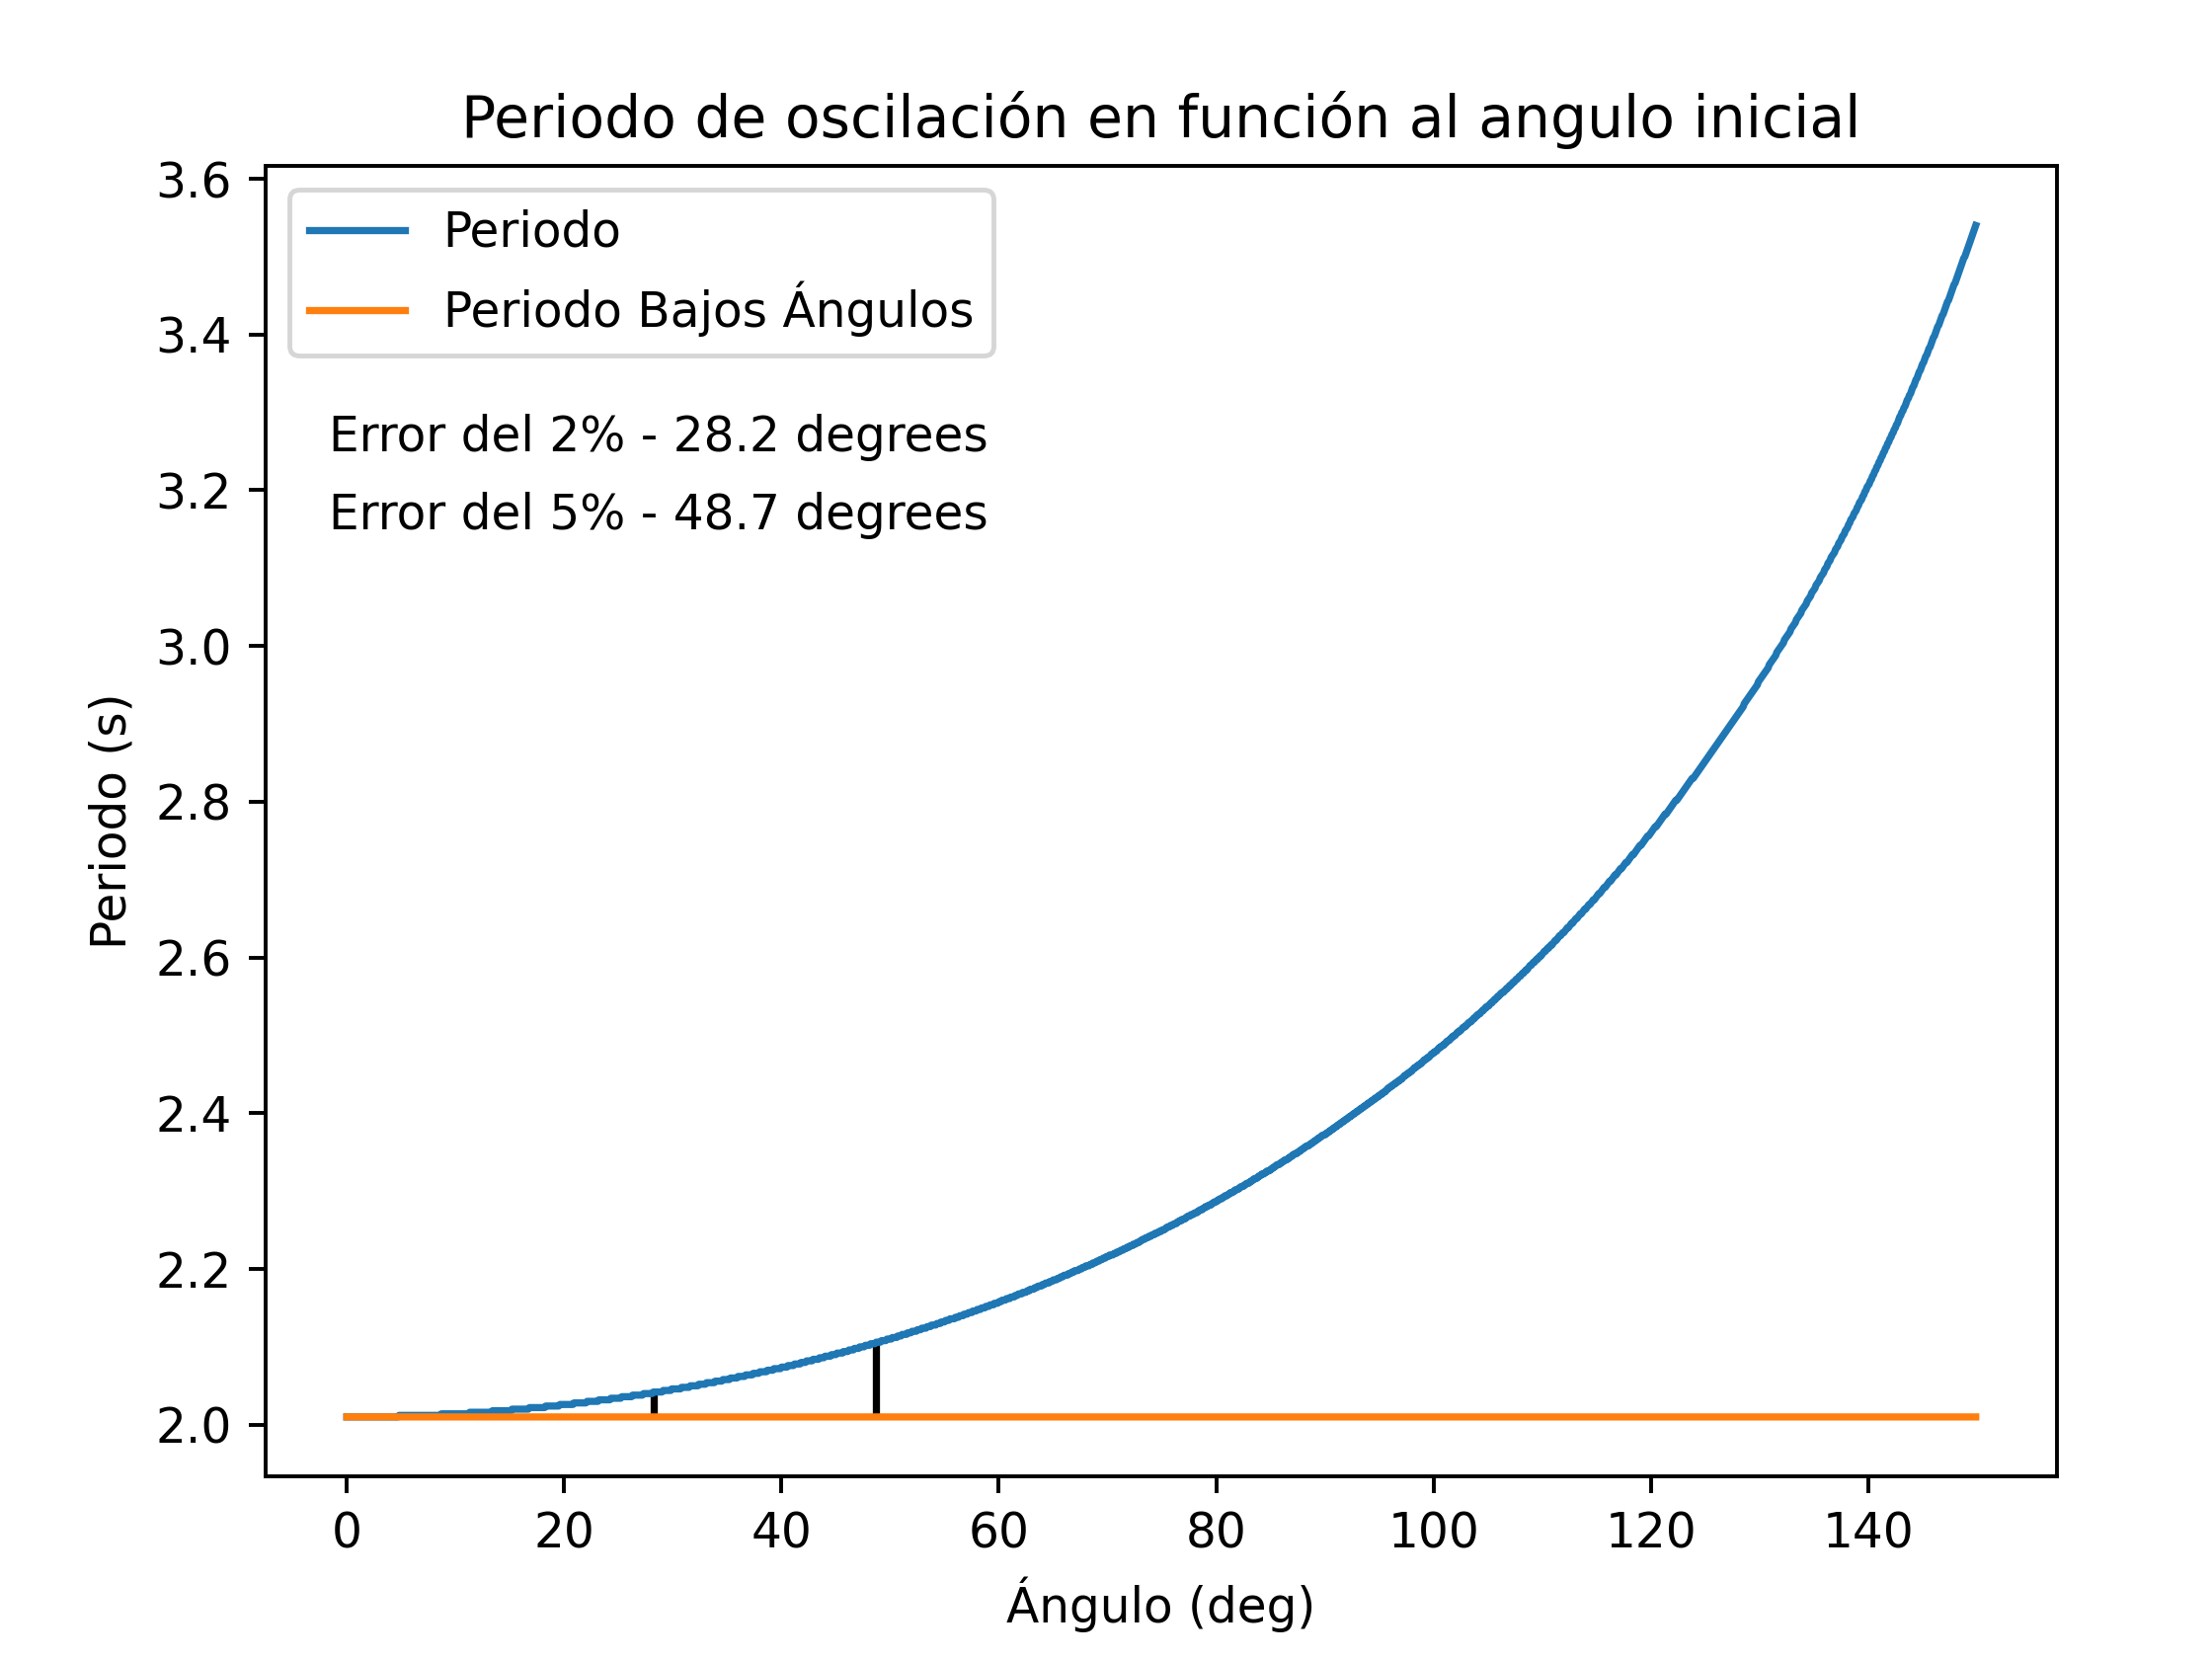
\includegraphics[width=.68\textwidth]{Fig4.png}
\end{wrapfigure}

\hfill \break \\   
Después de calcular el periodo con ambos métodos para distintos ángulos iniciales, obtenemos esta gráfica. Para obtener el periodo hay que tener en cuenta cuando el ángulo deja de tomar una dirección y cambia a la otra, y después multiplicarlo por dos. Si lo pensamos la derivada del ángulo (la velocidad angular) será 0 siempre que alcance un máximo, y el periodo será el tiempo que tarda el péndulo en alcanzar dos de estos máximos (ida y vuelta). \\ \\El programa también calcula cuando la solución numérica dista de más de un 2\% y 5\% de la de ángulos pequeños. Esto resulta ser a partir de 28.2 y 48.7 grados respectivamente. Estos resultados están en línea con lo ya estudiado, que la solución para ángulos pequeños es eso, para ángulos pequeños, y diferirá de la realidad en mayor grado cuanto mayor sea el ángulo incial que usemos.

\pagebreak
Código que calcula la gráfica:
\begin{adjustwidth}{-17pt}{-17pt}
\lstinputlisting[language=Python, firstline=1, lastline=61]{4.py}
\end{adjustwidth}
\pagebreak



% %----------------------------------------------------------------------------------------
% %	SECTION 6
% %----------------------------------------------------------------------------------------

\subsection{Cálculo de las energías en el péndulo}

\begin{wrapfigure}{l}{0.7\textwidth}
\centering
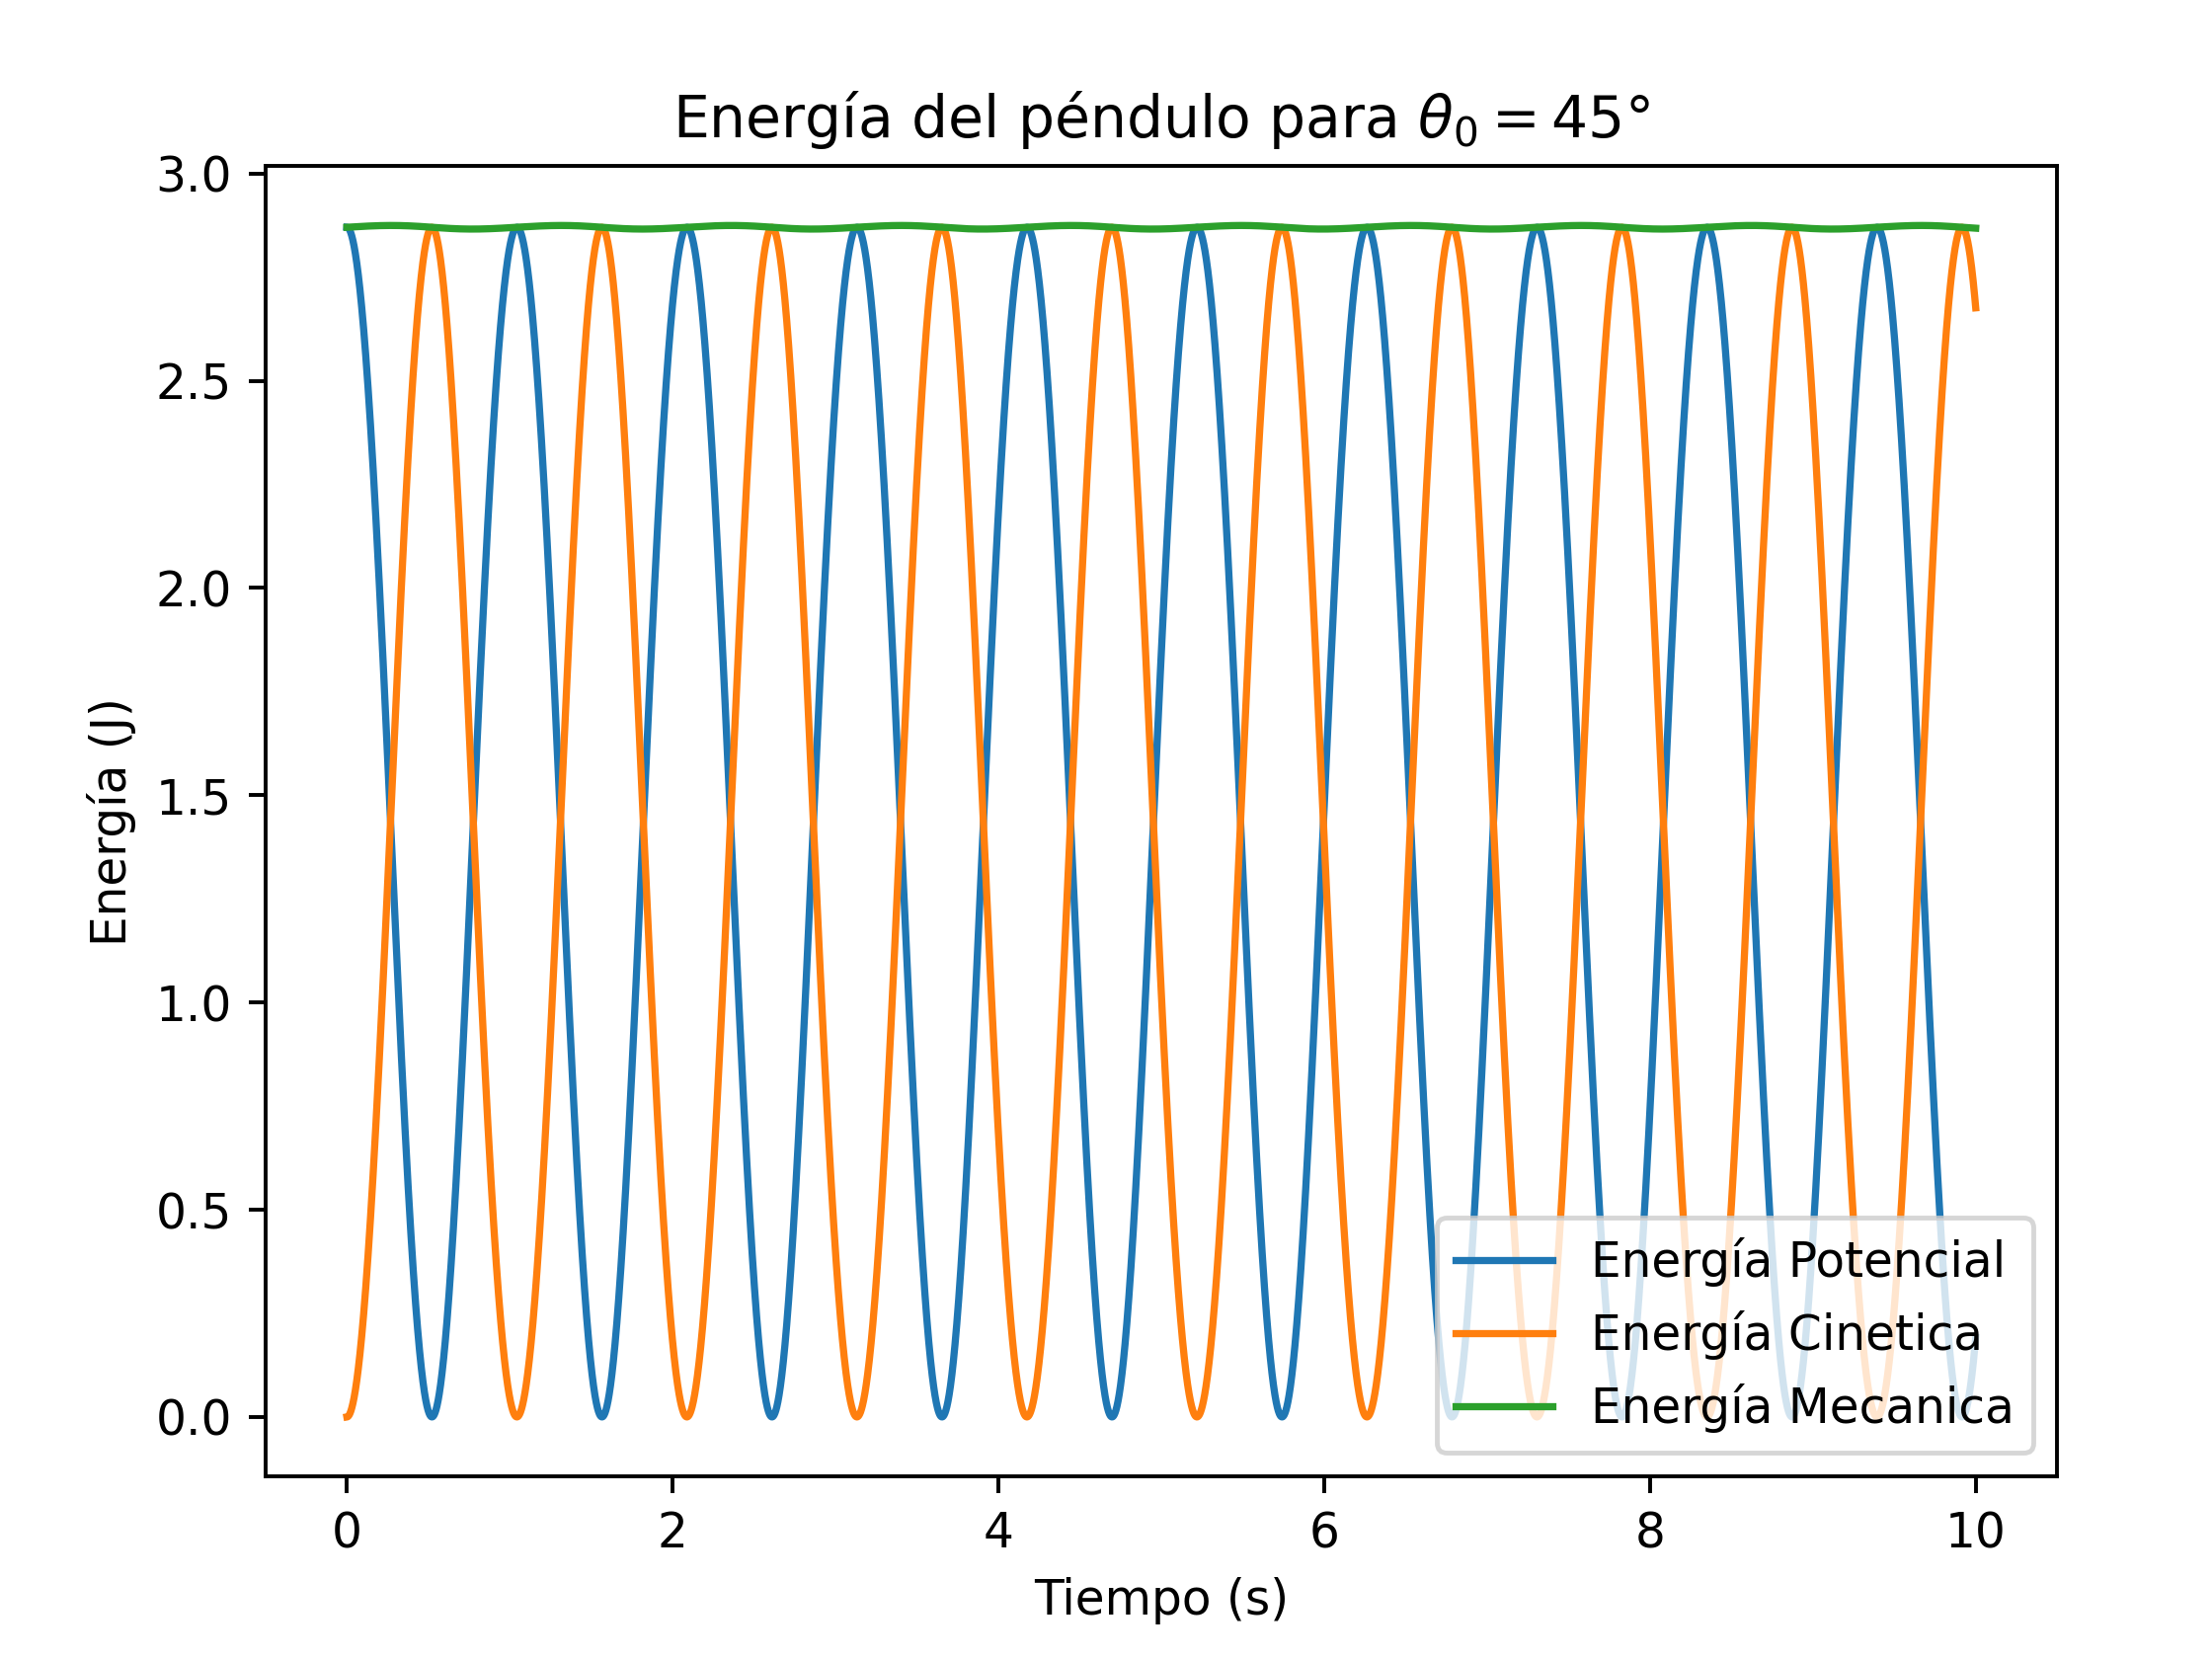
\includegraphics[width=.68\textwidth]{Fig5.png}
\end{wrapfigure}

\hfill \break \\
Tomando 10 segundos de la oscilación de un péndulo sin rozamiento que empezó a oscilar desde un ángulo de 45 grados, obtenemos esta gráfica para las energías. Observamos como inicialmente solo tiene energía potencial, y la energía cinética es cero. Conforme avanza el tiempo, estas dos se intercambian siempre estando a media fase de distancia entre sí. De esta forma, la suma de ellas en cada instante, la energía mecánica, tendrá un valor constante que en este caso ronda los 2.8J

\hfill \break \\
Código que calcula la gráfica:
\lstinputlisting[language=Python, firstline=1, lastline=32]{5.py}
\pagebreak

% %----------------------------------------------------------------------------------------
% %	SECTION 7
% %----------------------------------------------------------------------------------------
\section{Parte b) - Péndulo con Fricción}

\subsection{Cálculo del Ángulo y la Velocidad Angular}
\begin{figure}[h]
\centering
\hspace*{-2.3cm}
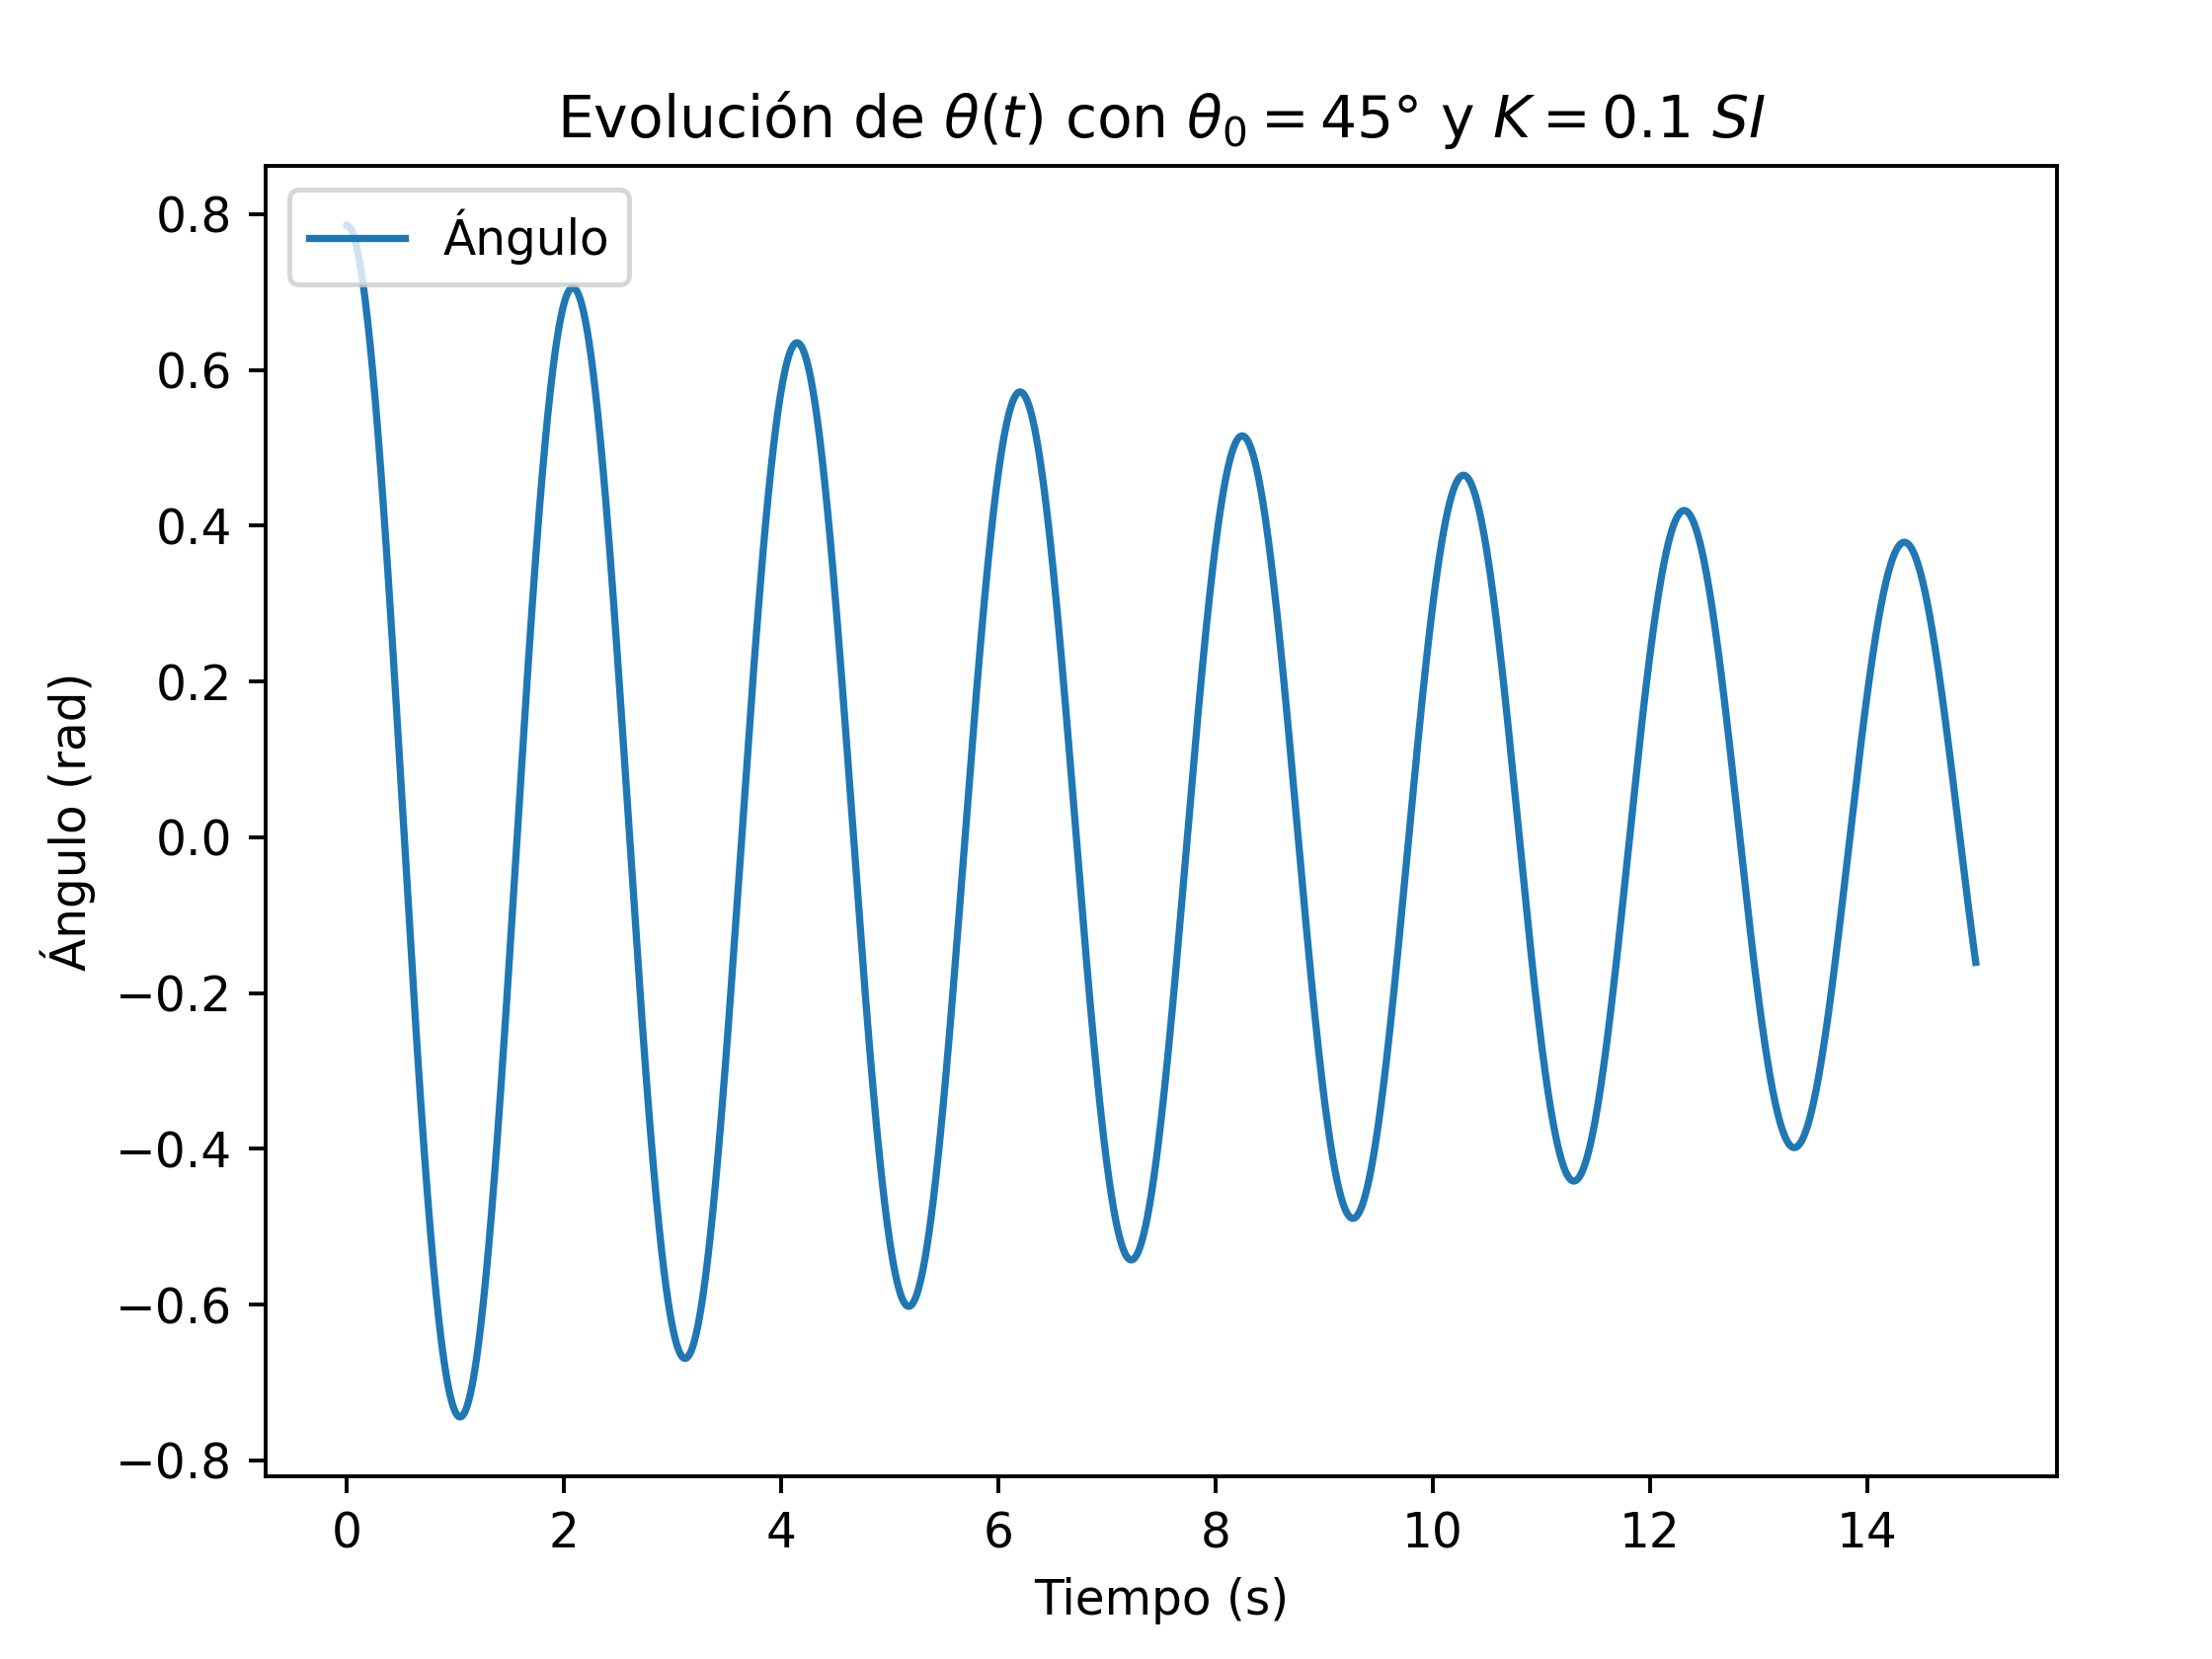
\includegraphics[width=.57\textwidth]{Fig6a.png}\hfill
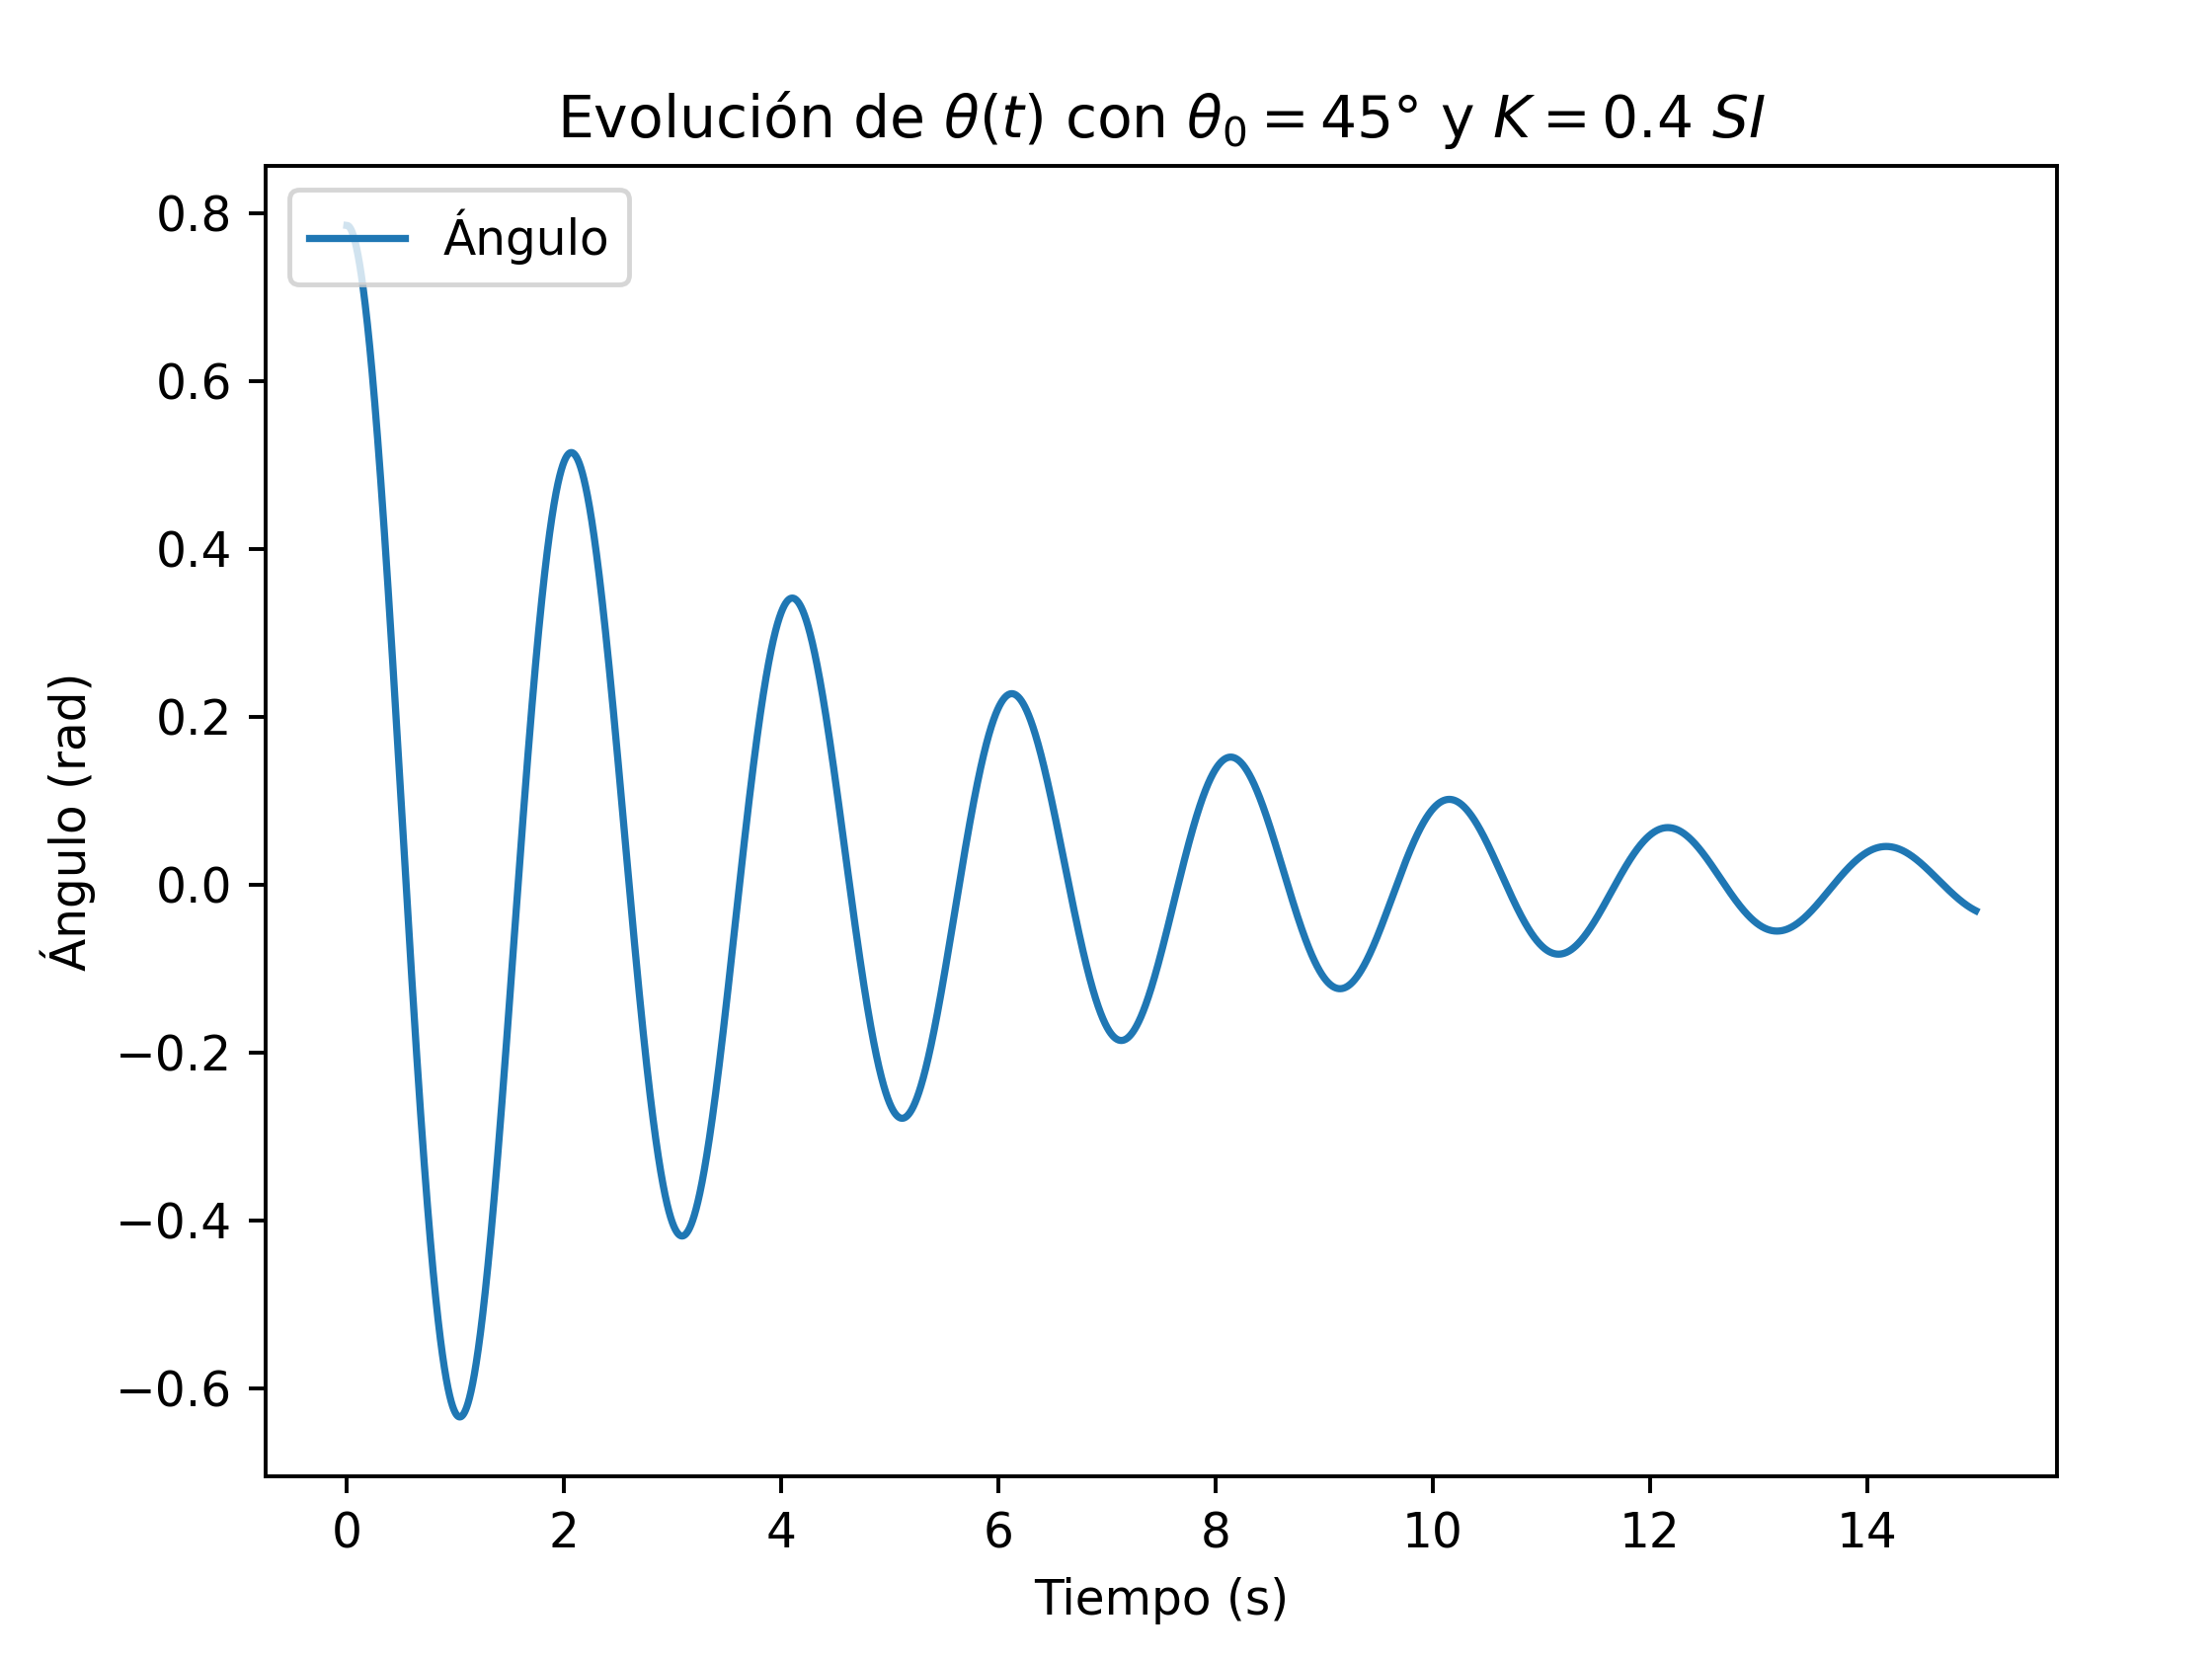
\includegraphics[width=.57\textwidth]{Fig7a.png}
\hspace*{-2.3cm}
\end{figure}
\begin{figure}[h]
\centering
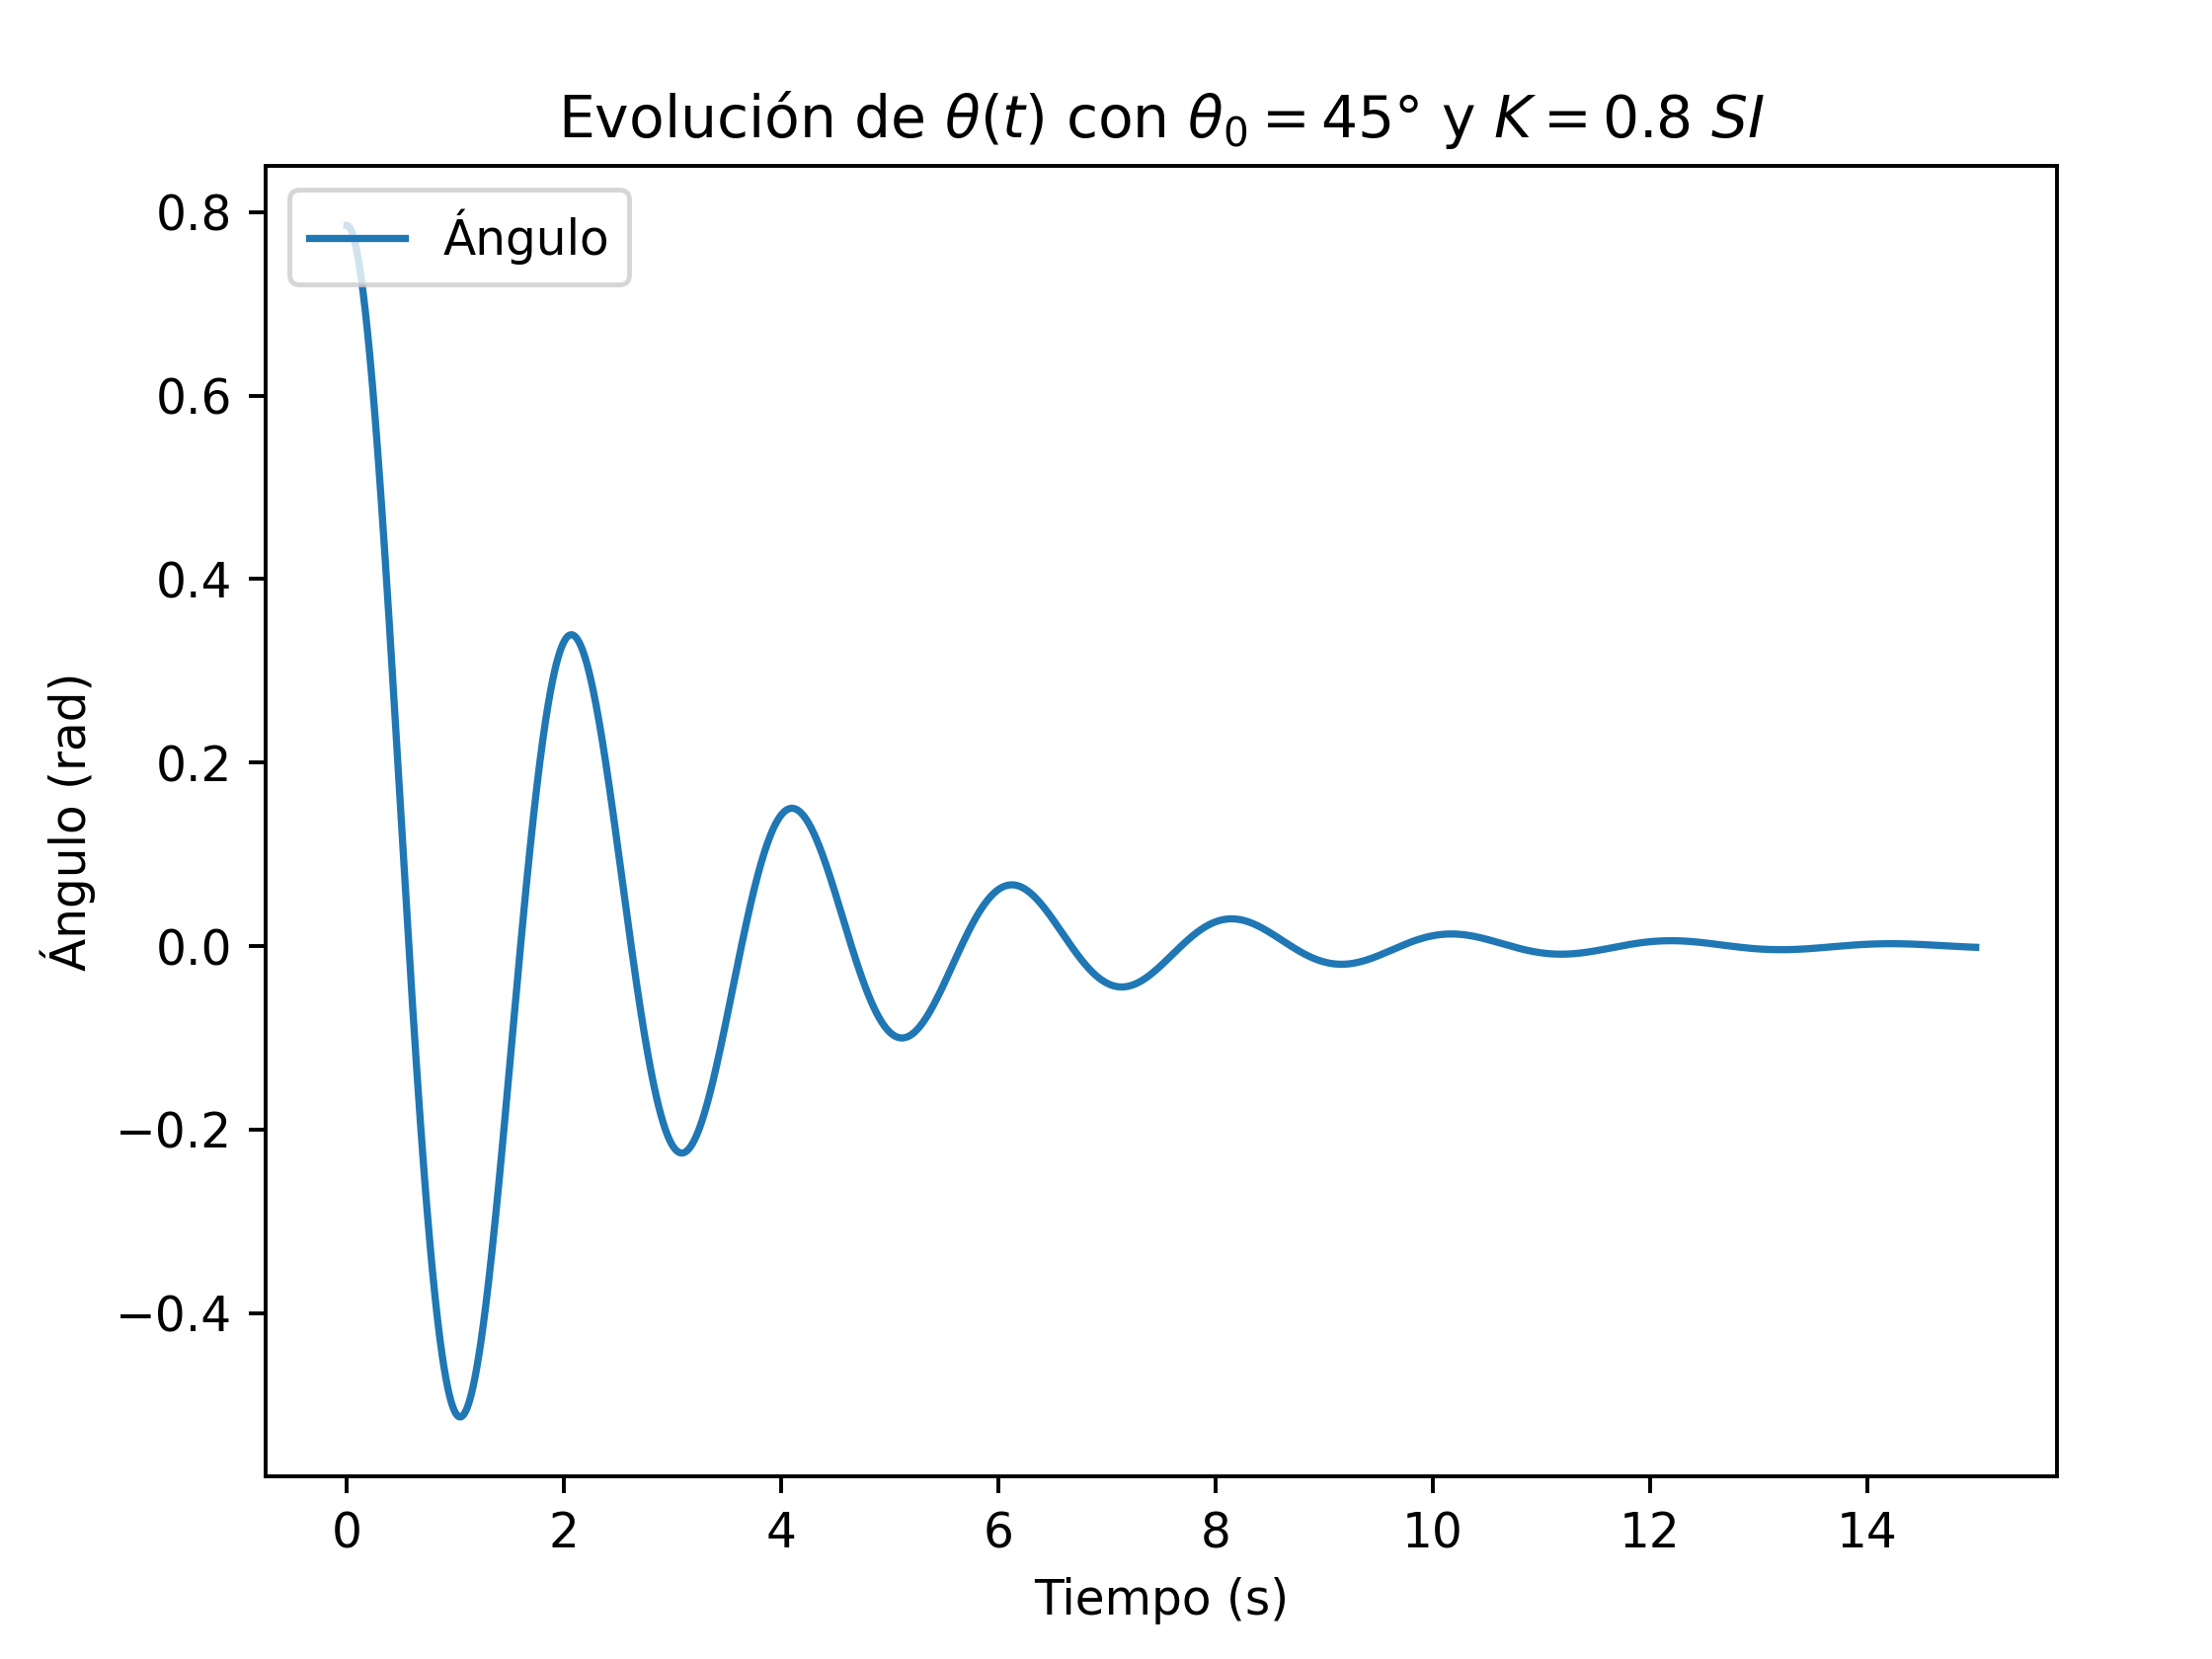
\includegraphics[width=.57\textwidth]{Fig8a.png}
\end{figure}

\hfill \break \\
Observamos como un péndulo soltado desde el mismo ángulo inicial, 45 grados, y estudiado con diferentes valores para la K durante 15 segundos, el ángulo máximo que descrirá el péndulo será siempre el ángulo inicial, ya que conforme pase el tiempo las oscilaciones cada vez serán de menor tamaño. \\\\Y es que para valores de K muy grandes, como es 0.8 en la última figura, en la primera oscilación no llega a alcanzar ni la mitad del ángulo desde el que se soltó, ya que la mayor parte de la energía potencial ha sido disipada.

\pagebreak

\begin{figure}[h]
\centering
\hspace*{-2.3cm}
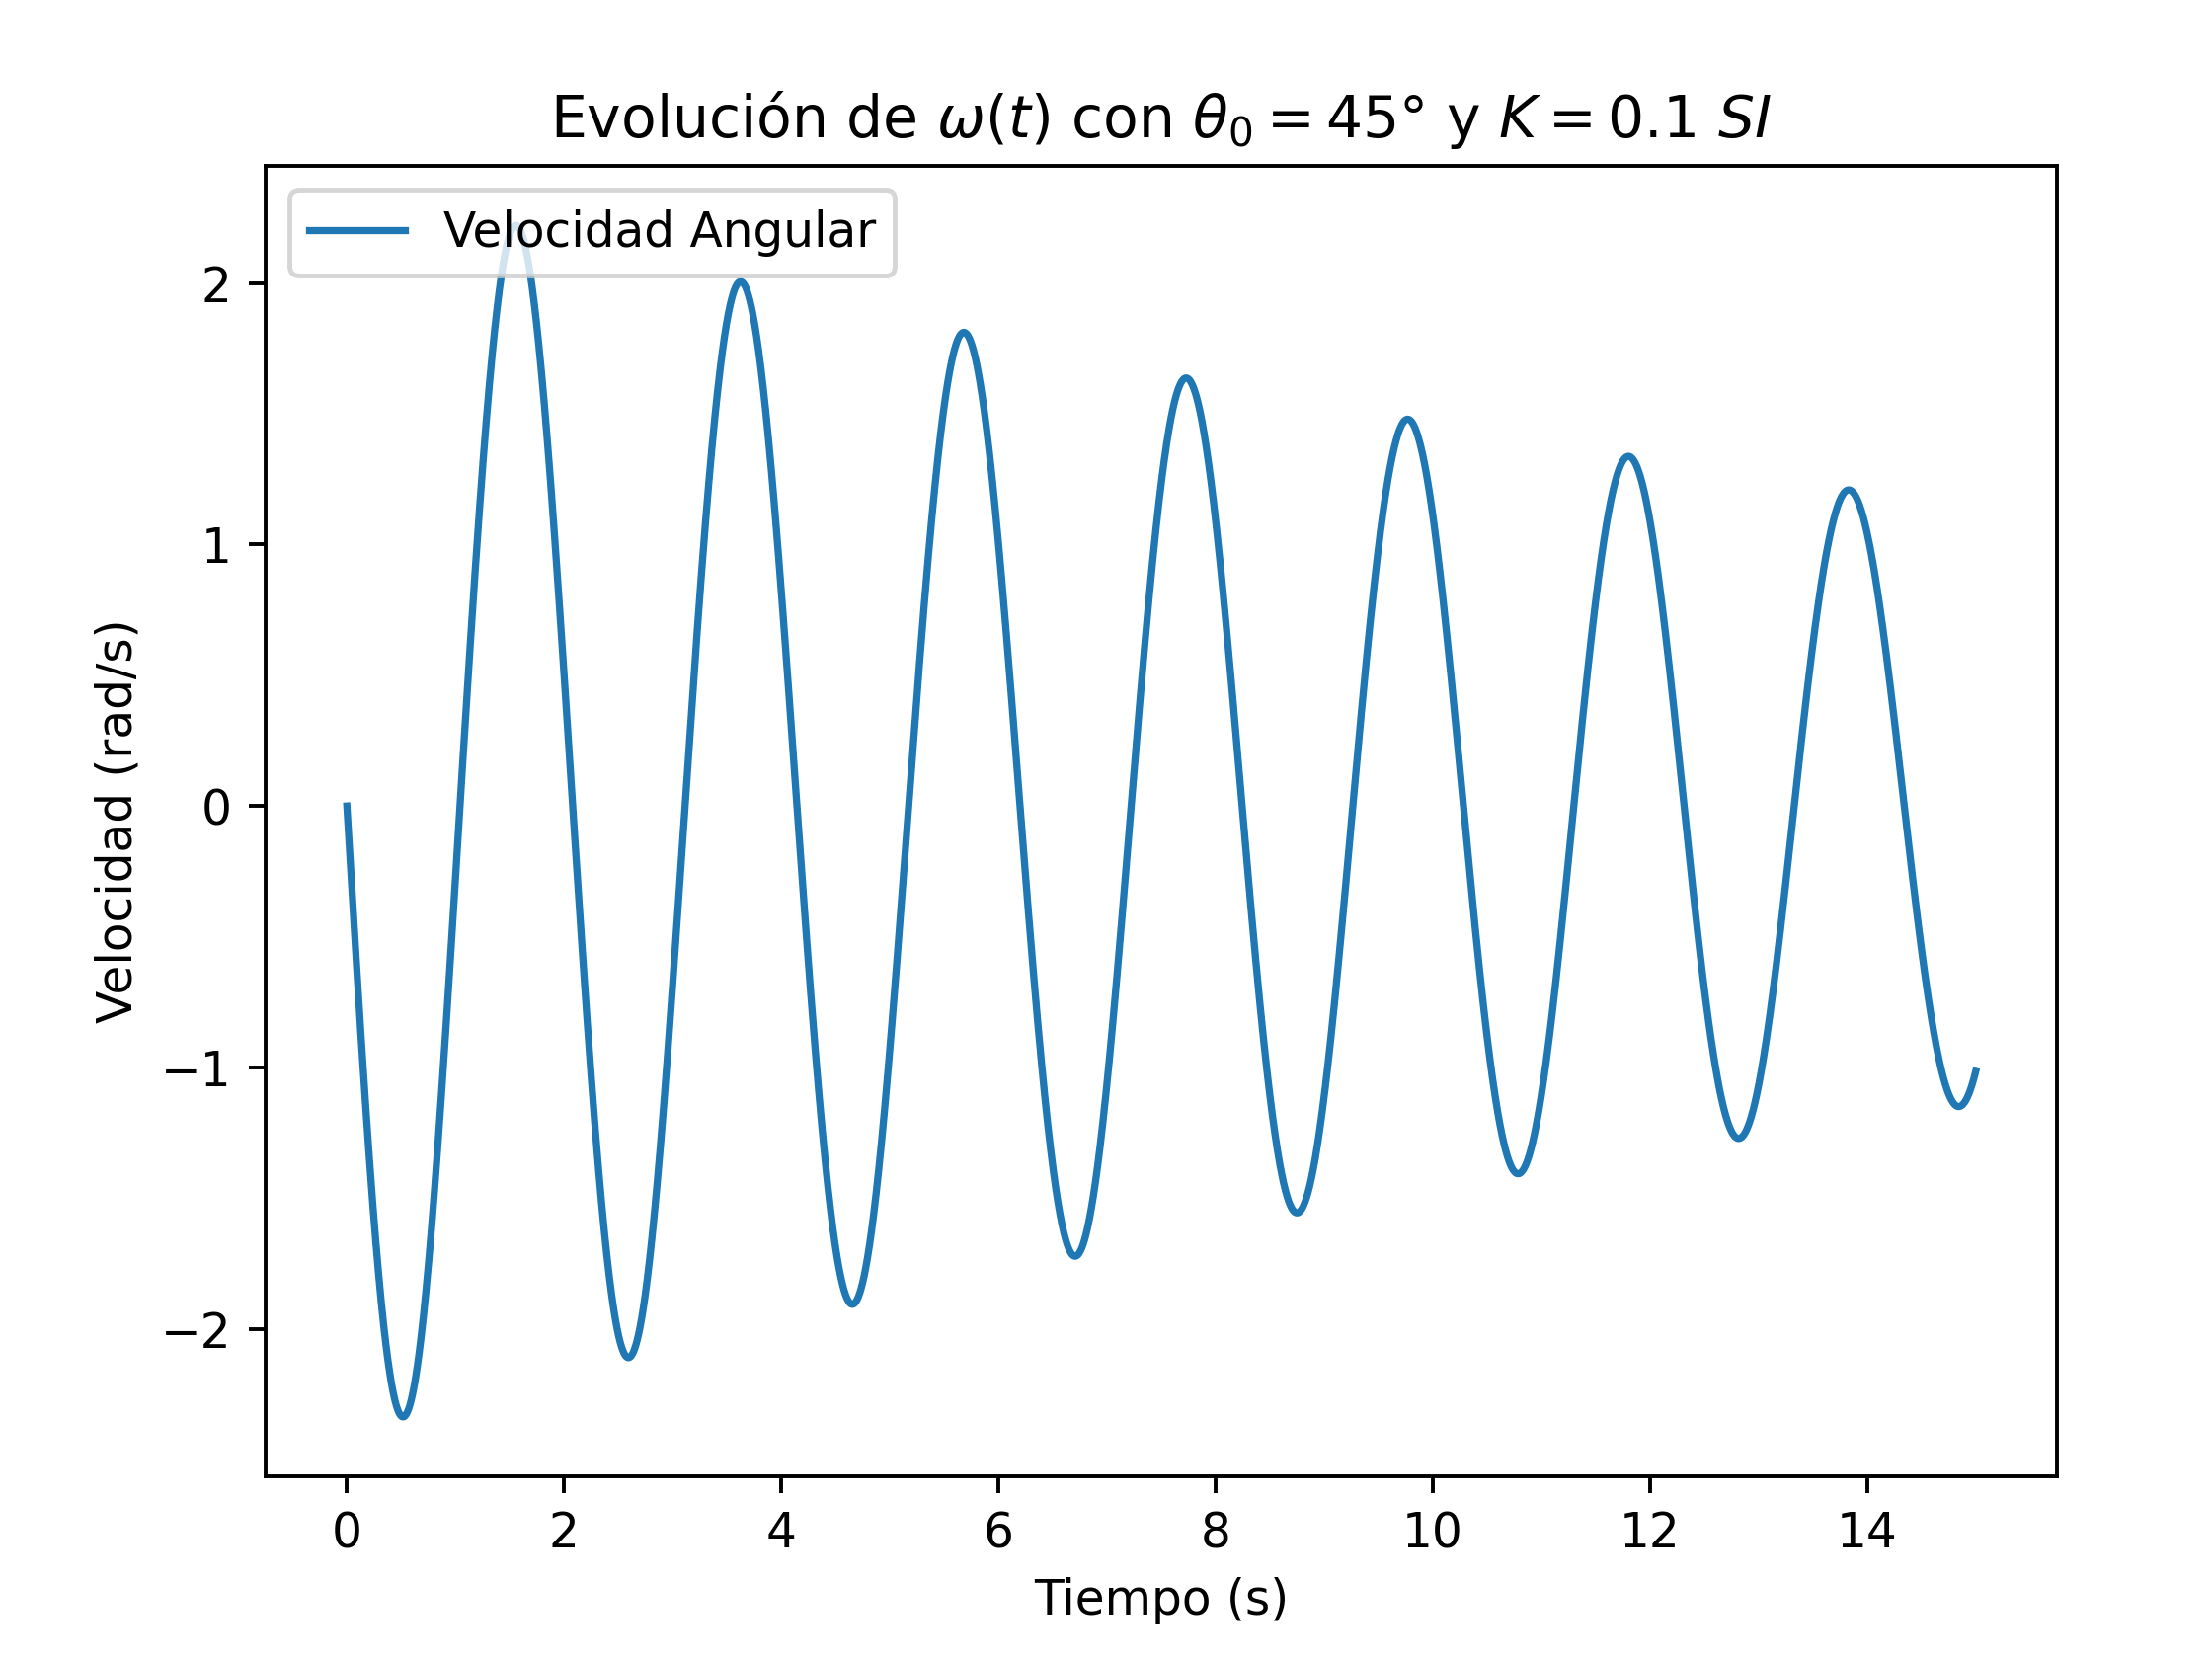
\includegraphics[width=.57\textwidth]{Fig6b.png}\hfill
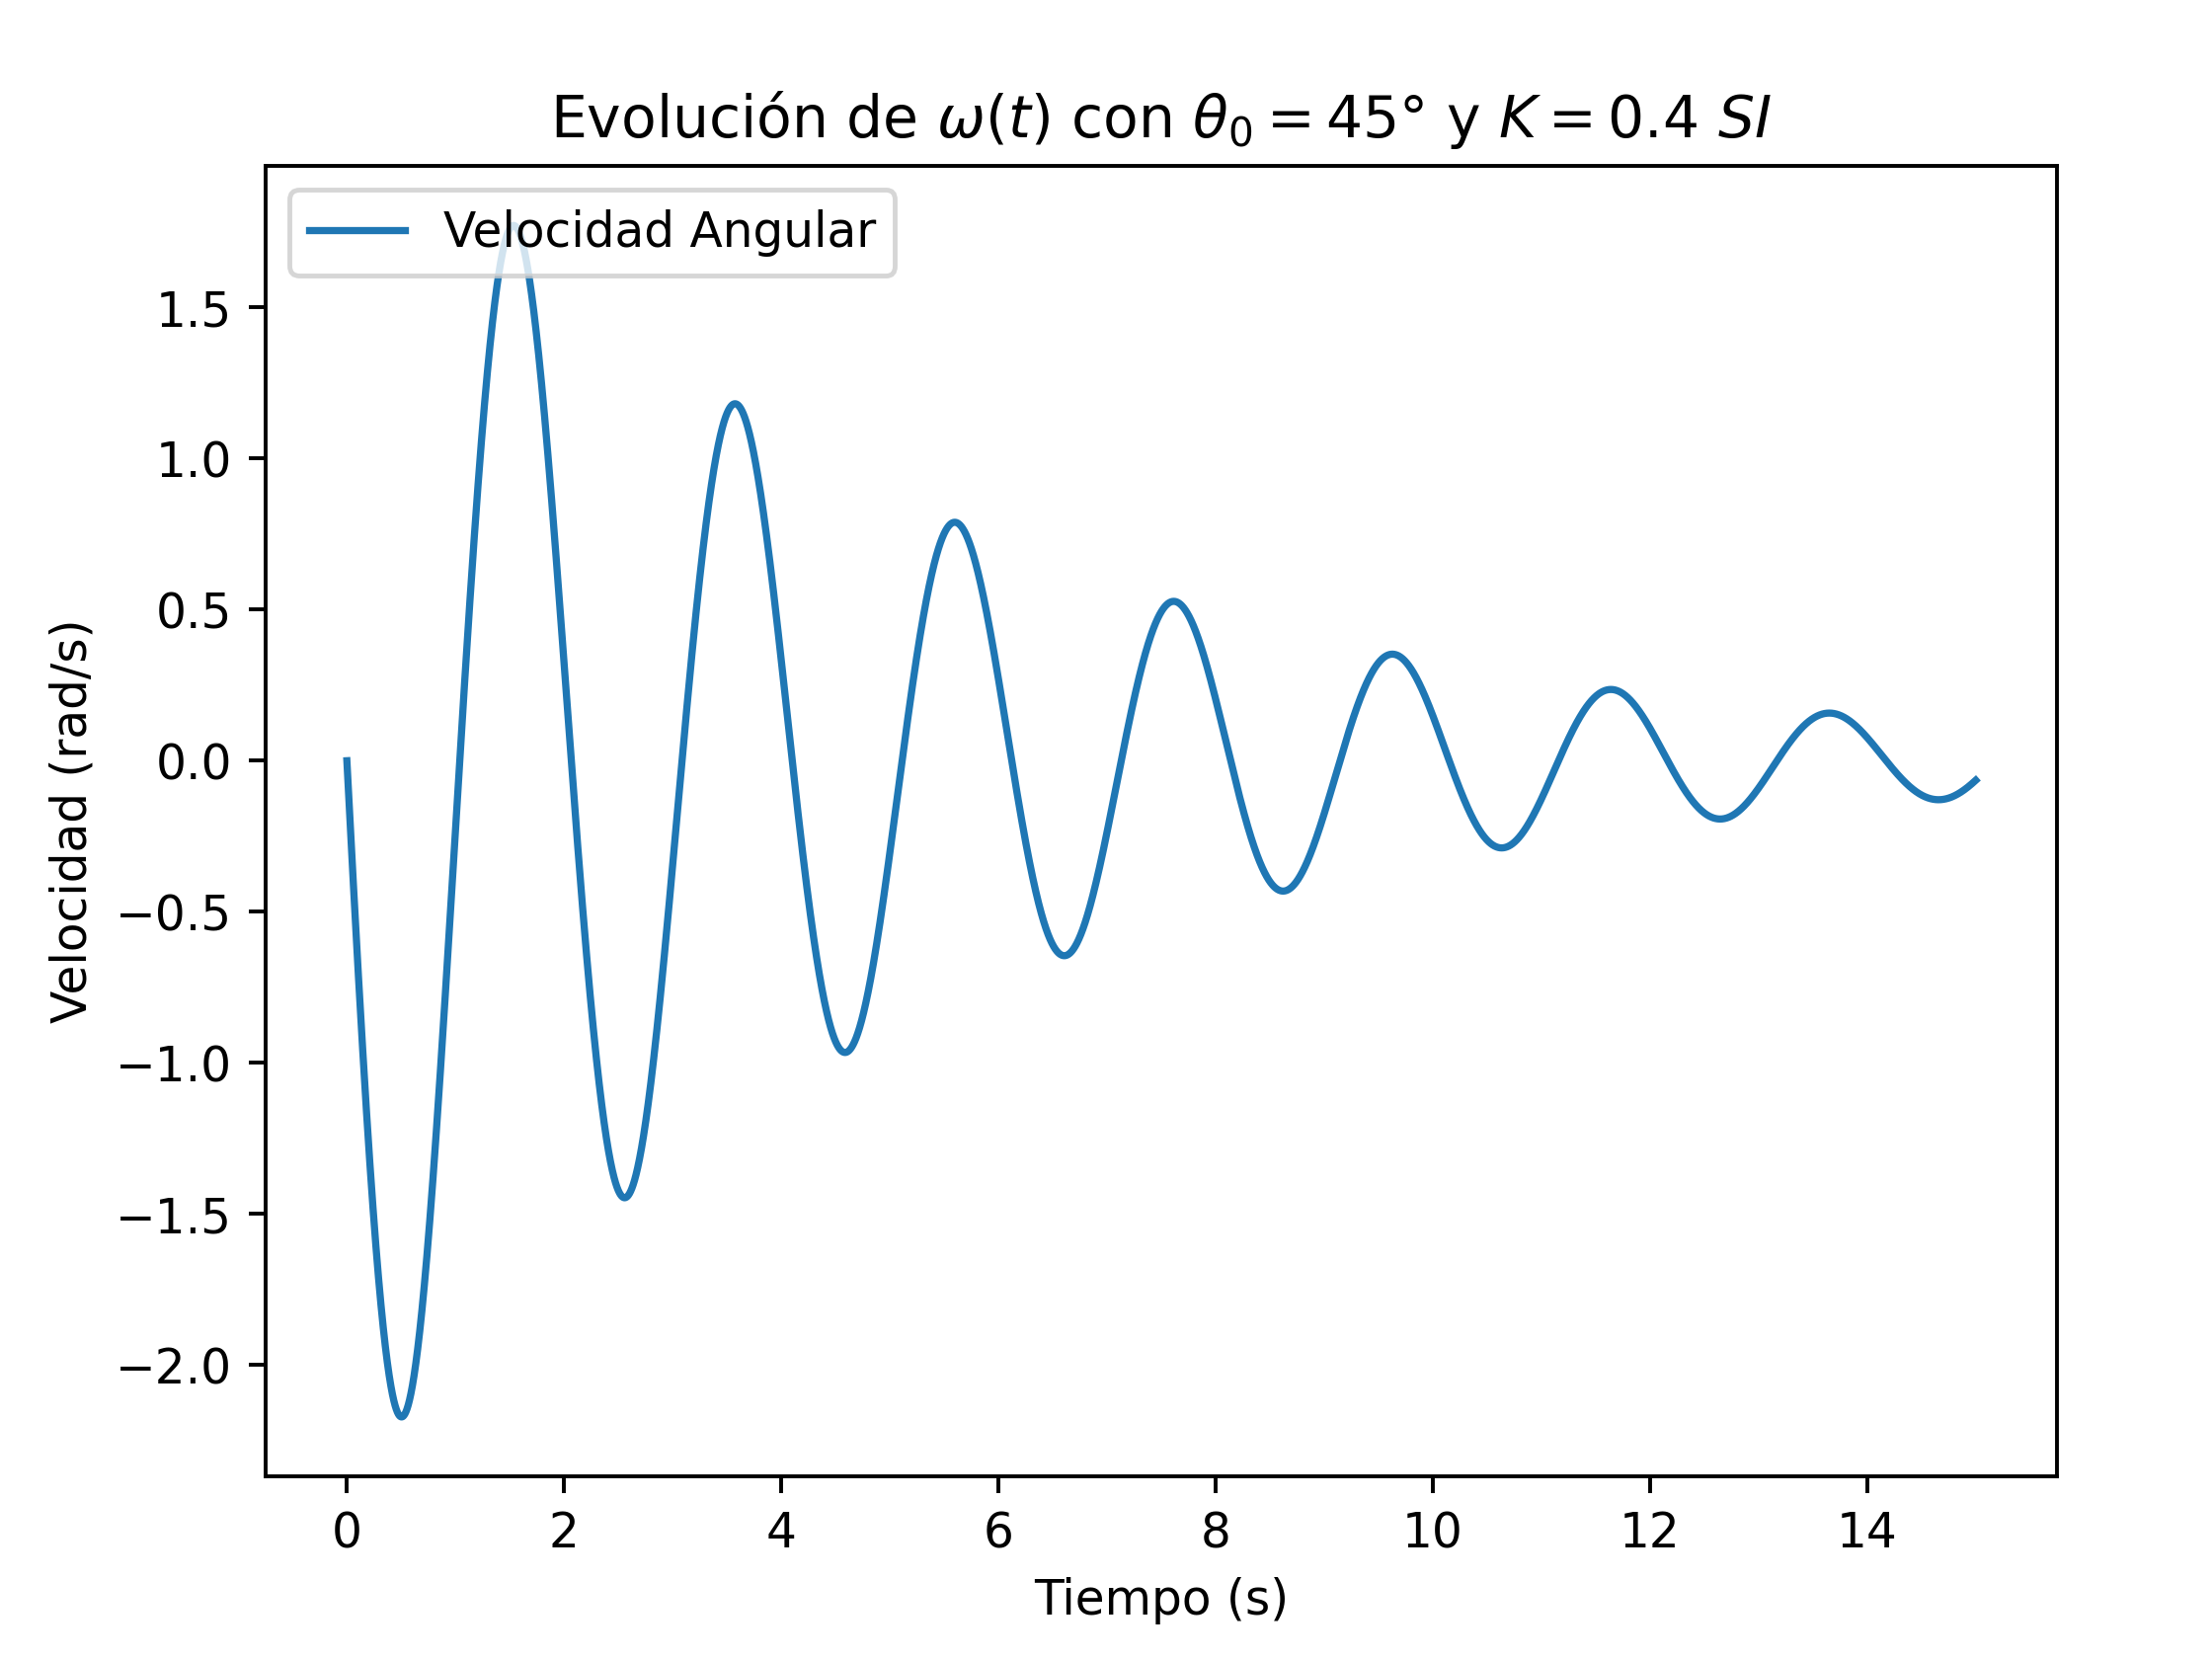
\includegraphics[width=.57\textwidth]{Fig7b.png}
\hspace*{-2.3cm}
\end{figure}
\begin{figure}[h]
\centering
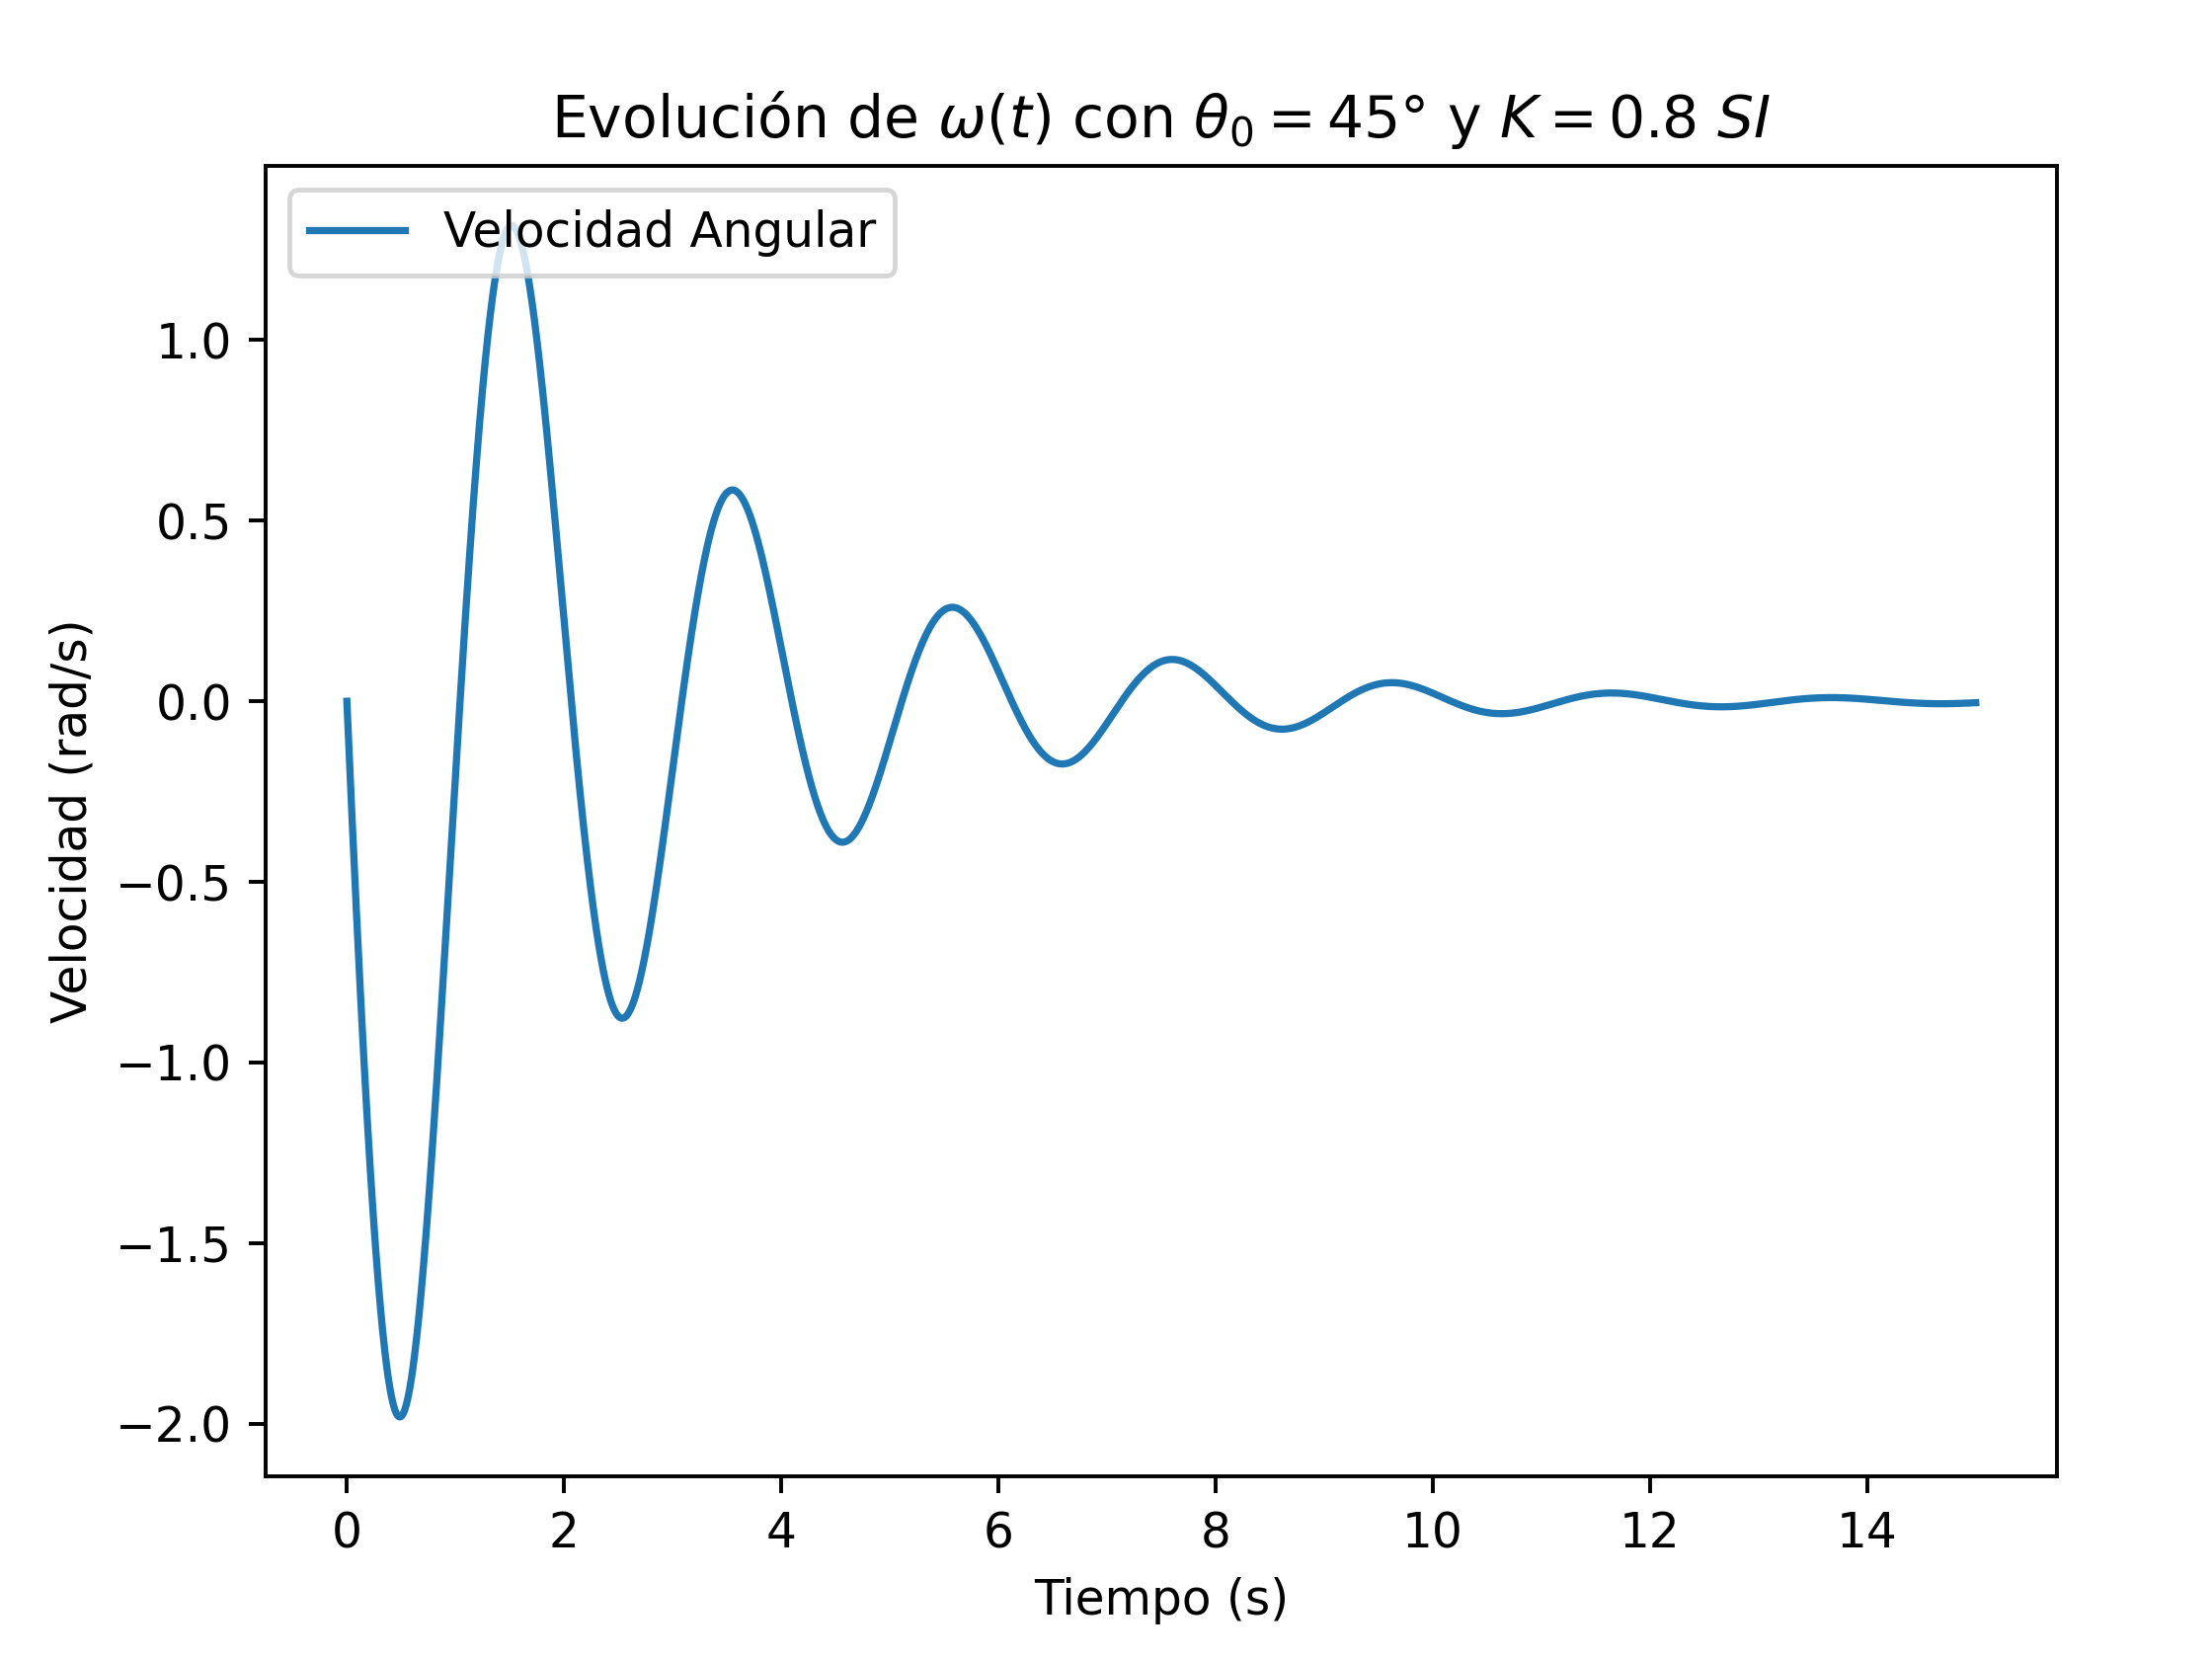
\includegraphics[width=.57\textwidth]{Fig8b.png}
\end{figure}

\hfill \break \\
Observamos aquí la velocidad angular para el mismo caso observado con el ángulo, un péndulo soltado desde 45 grados y graficado durante 15 segundos para varios valores de K. \\ \\Al igual que con el ángulo, la velocidad angular alcanzará su pico máximo en la primera oscilación (no en el instante $t=0$ ya que ahí $\omega = 0$) y irá descendiendo en mayor o menor grado en función del tamaño de la K utilizada.

\pagebreak
\hfill \break \\
\hfill \break \\
\hfill \break \\

Código que calcula las gráficas:
\begin{adjustwidth}{-12pt}{-12pt}
\lstinputlisting[language=Python, firstline=1, lastline=34]{6.py}
\end{adjustwidth}

\hfill \break \\
\hfill \break \\
Este código calcula tanto la velocidad angular como el ángulo en un solo código. El programa pregunta por un ángulo inicial y una K, y calcula ambas gráficas.
\pagebreak


\subsection{Cálculo de las energías}

\begin{figure}[h]
\centering
\hspace*{-2.3cm}
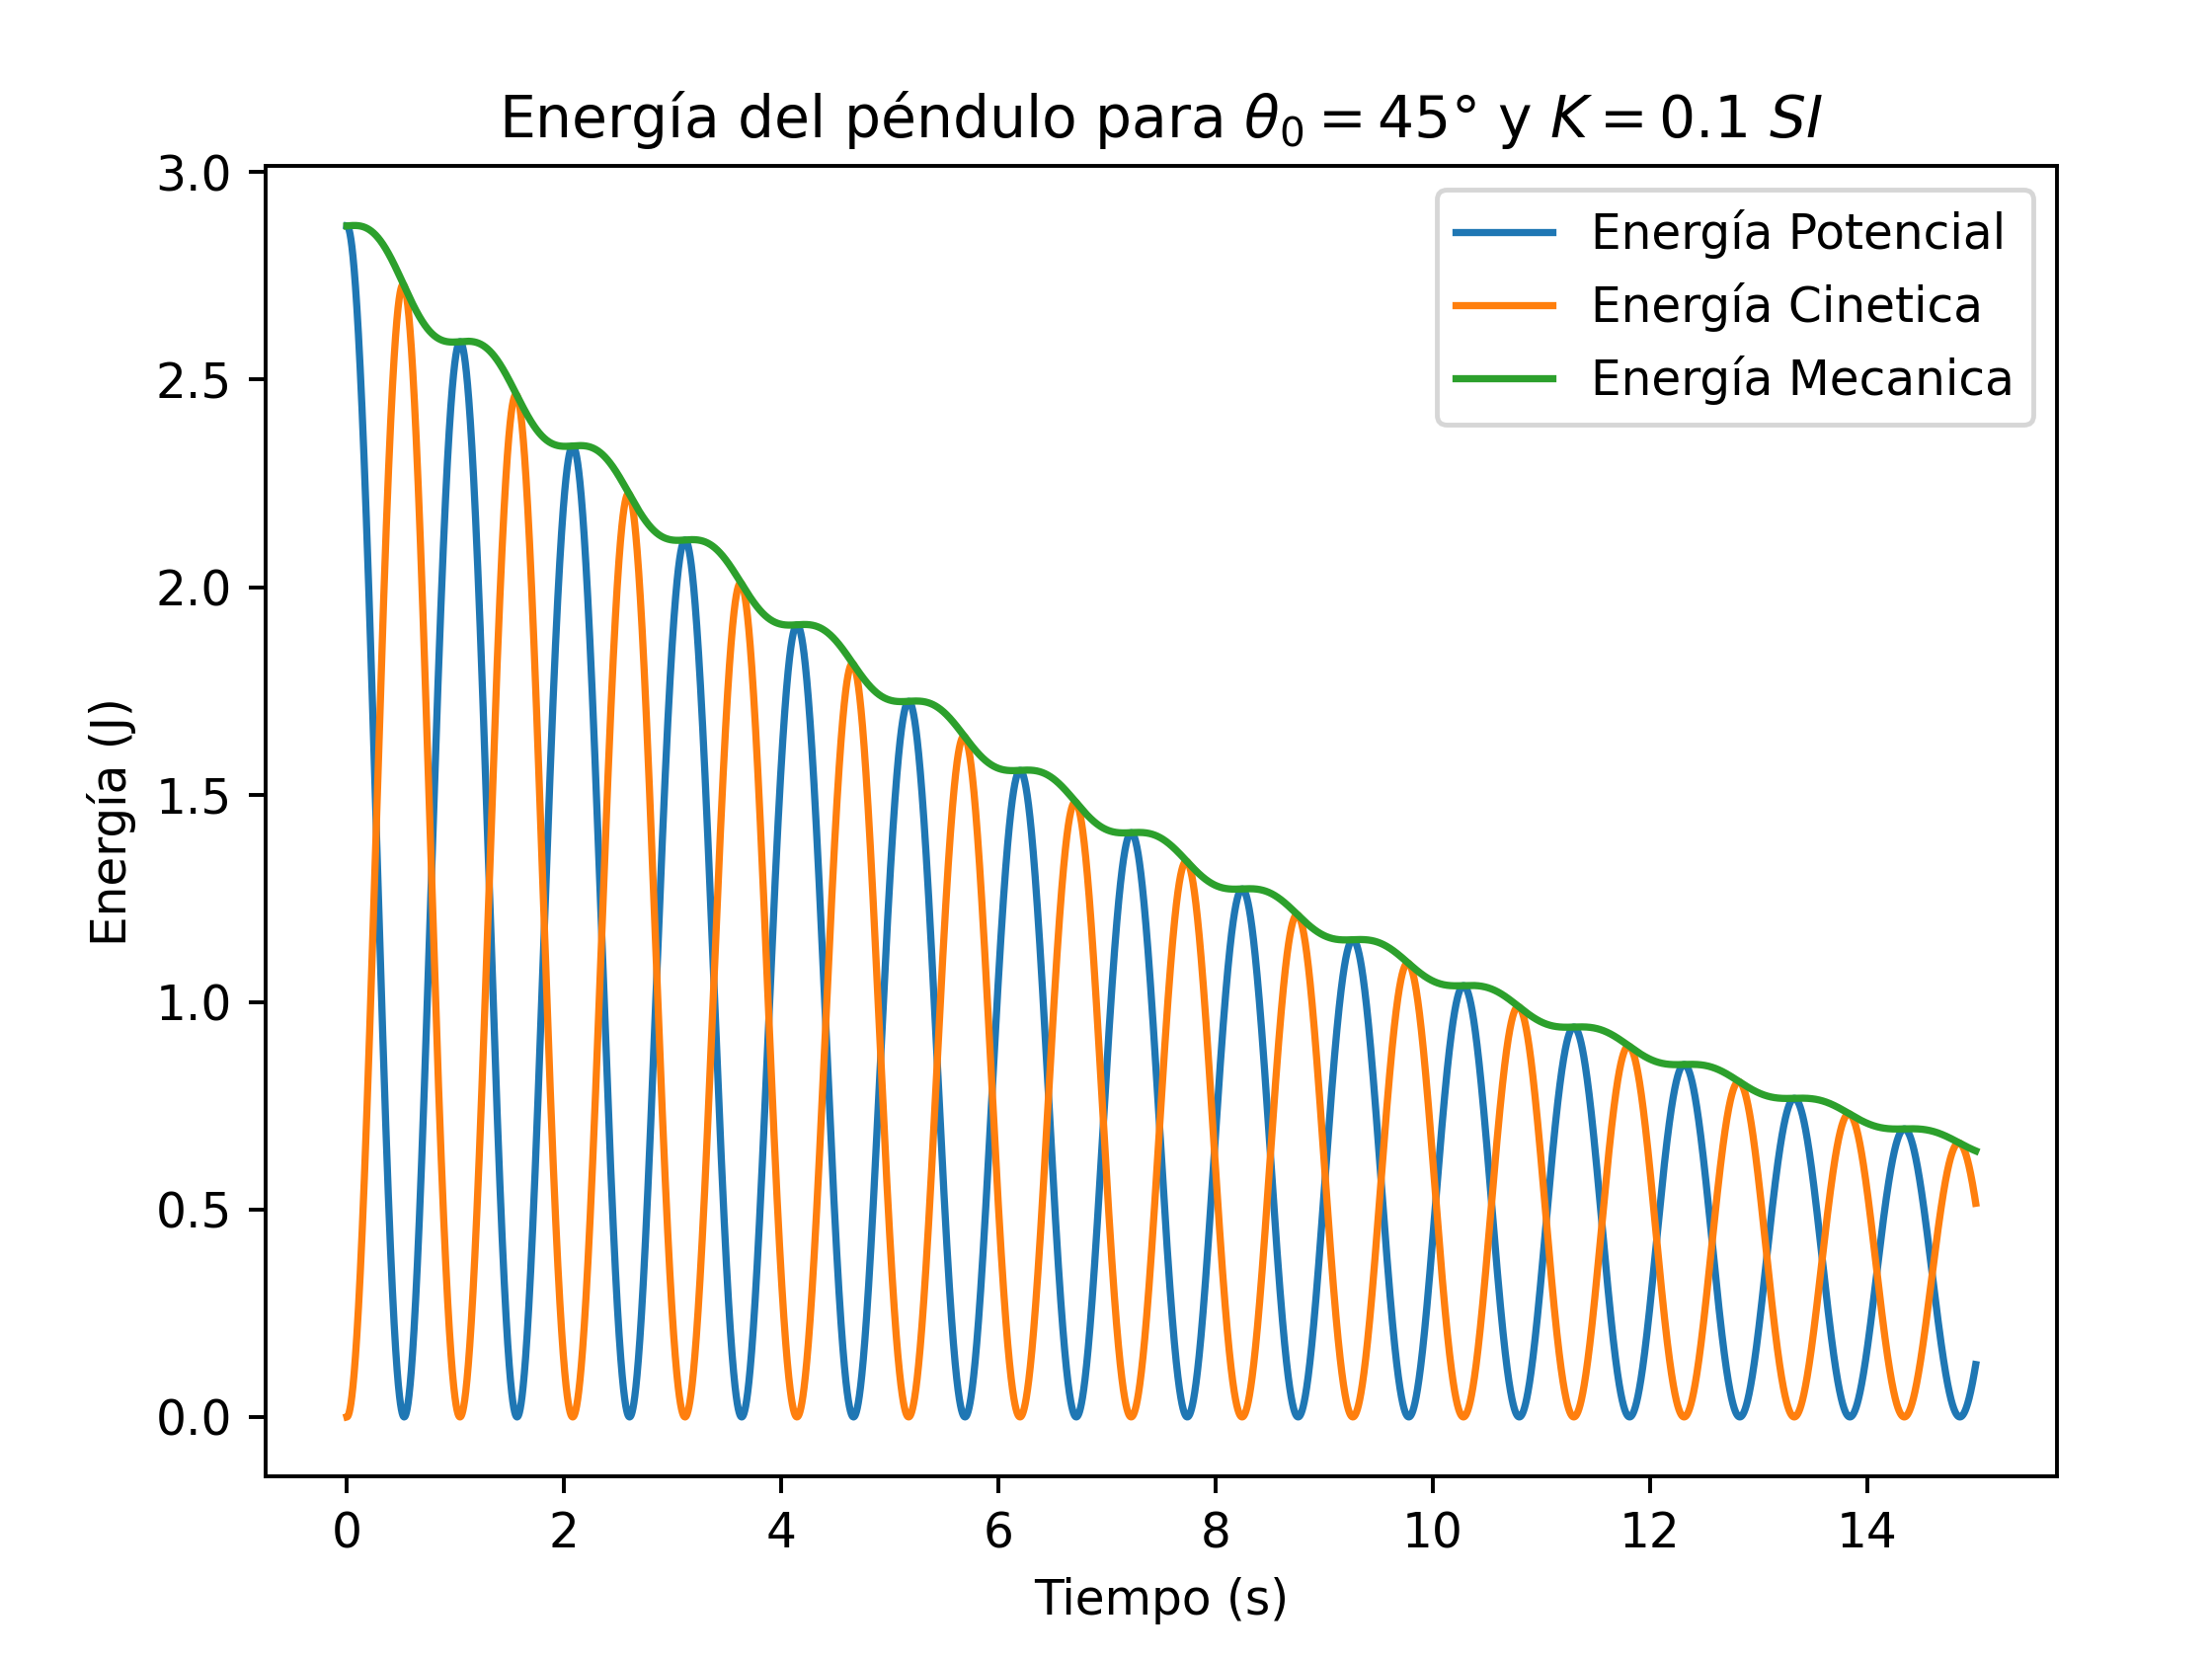
\includegraphics[width=.57\textwidth]{Fig9.png}\hfill
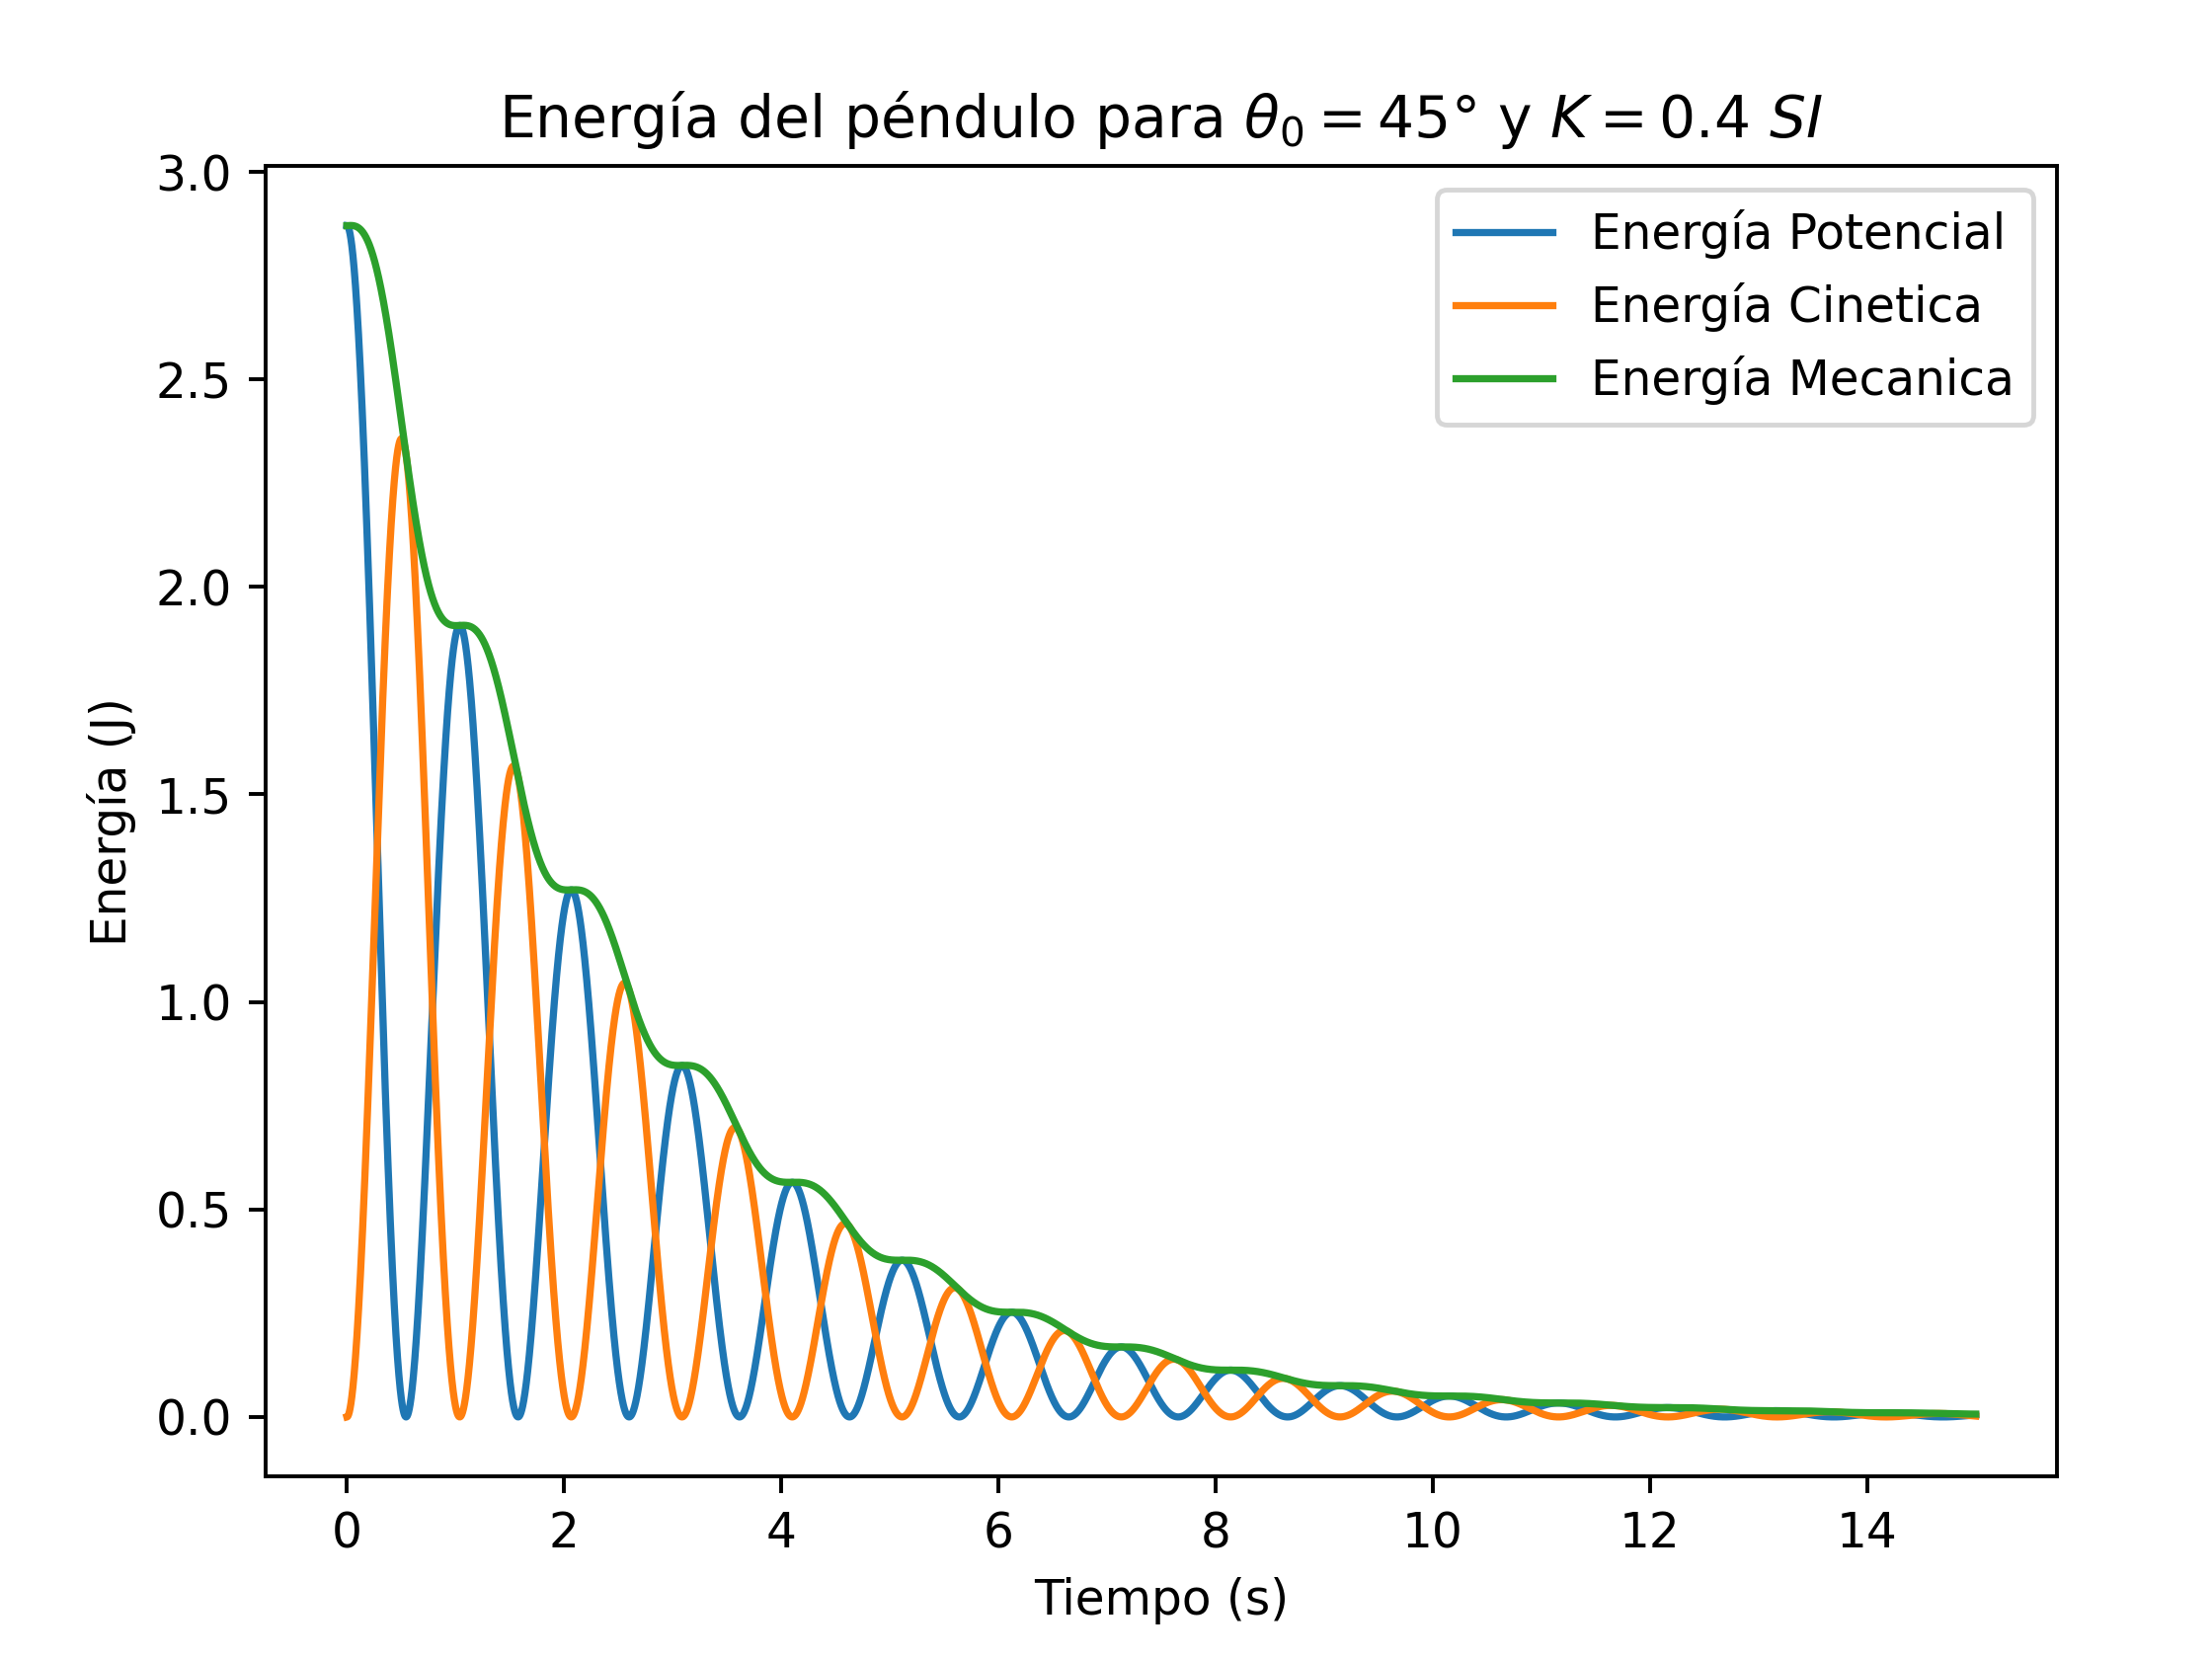
\includegraphics[width=.57\textwidth]{Fig10.png}
\hspace*{-2.3cm}
\end{figure}
\begin{figure}[h]
\centering
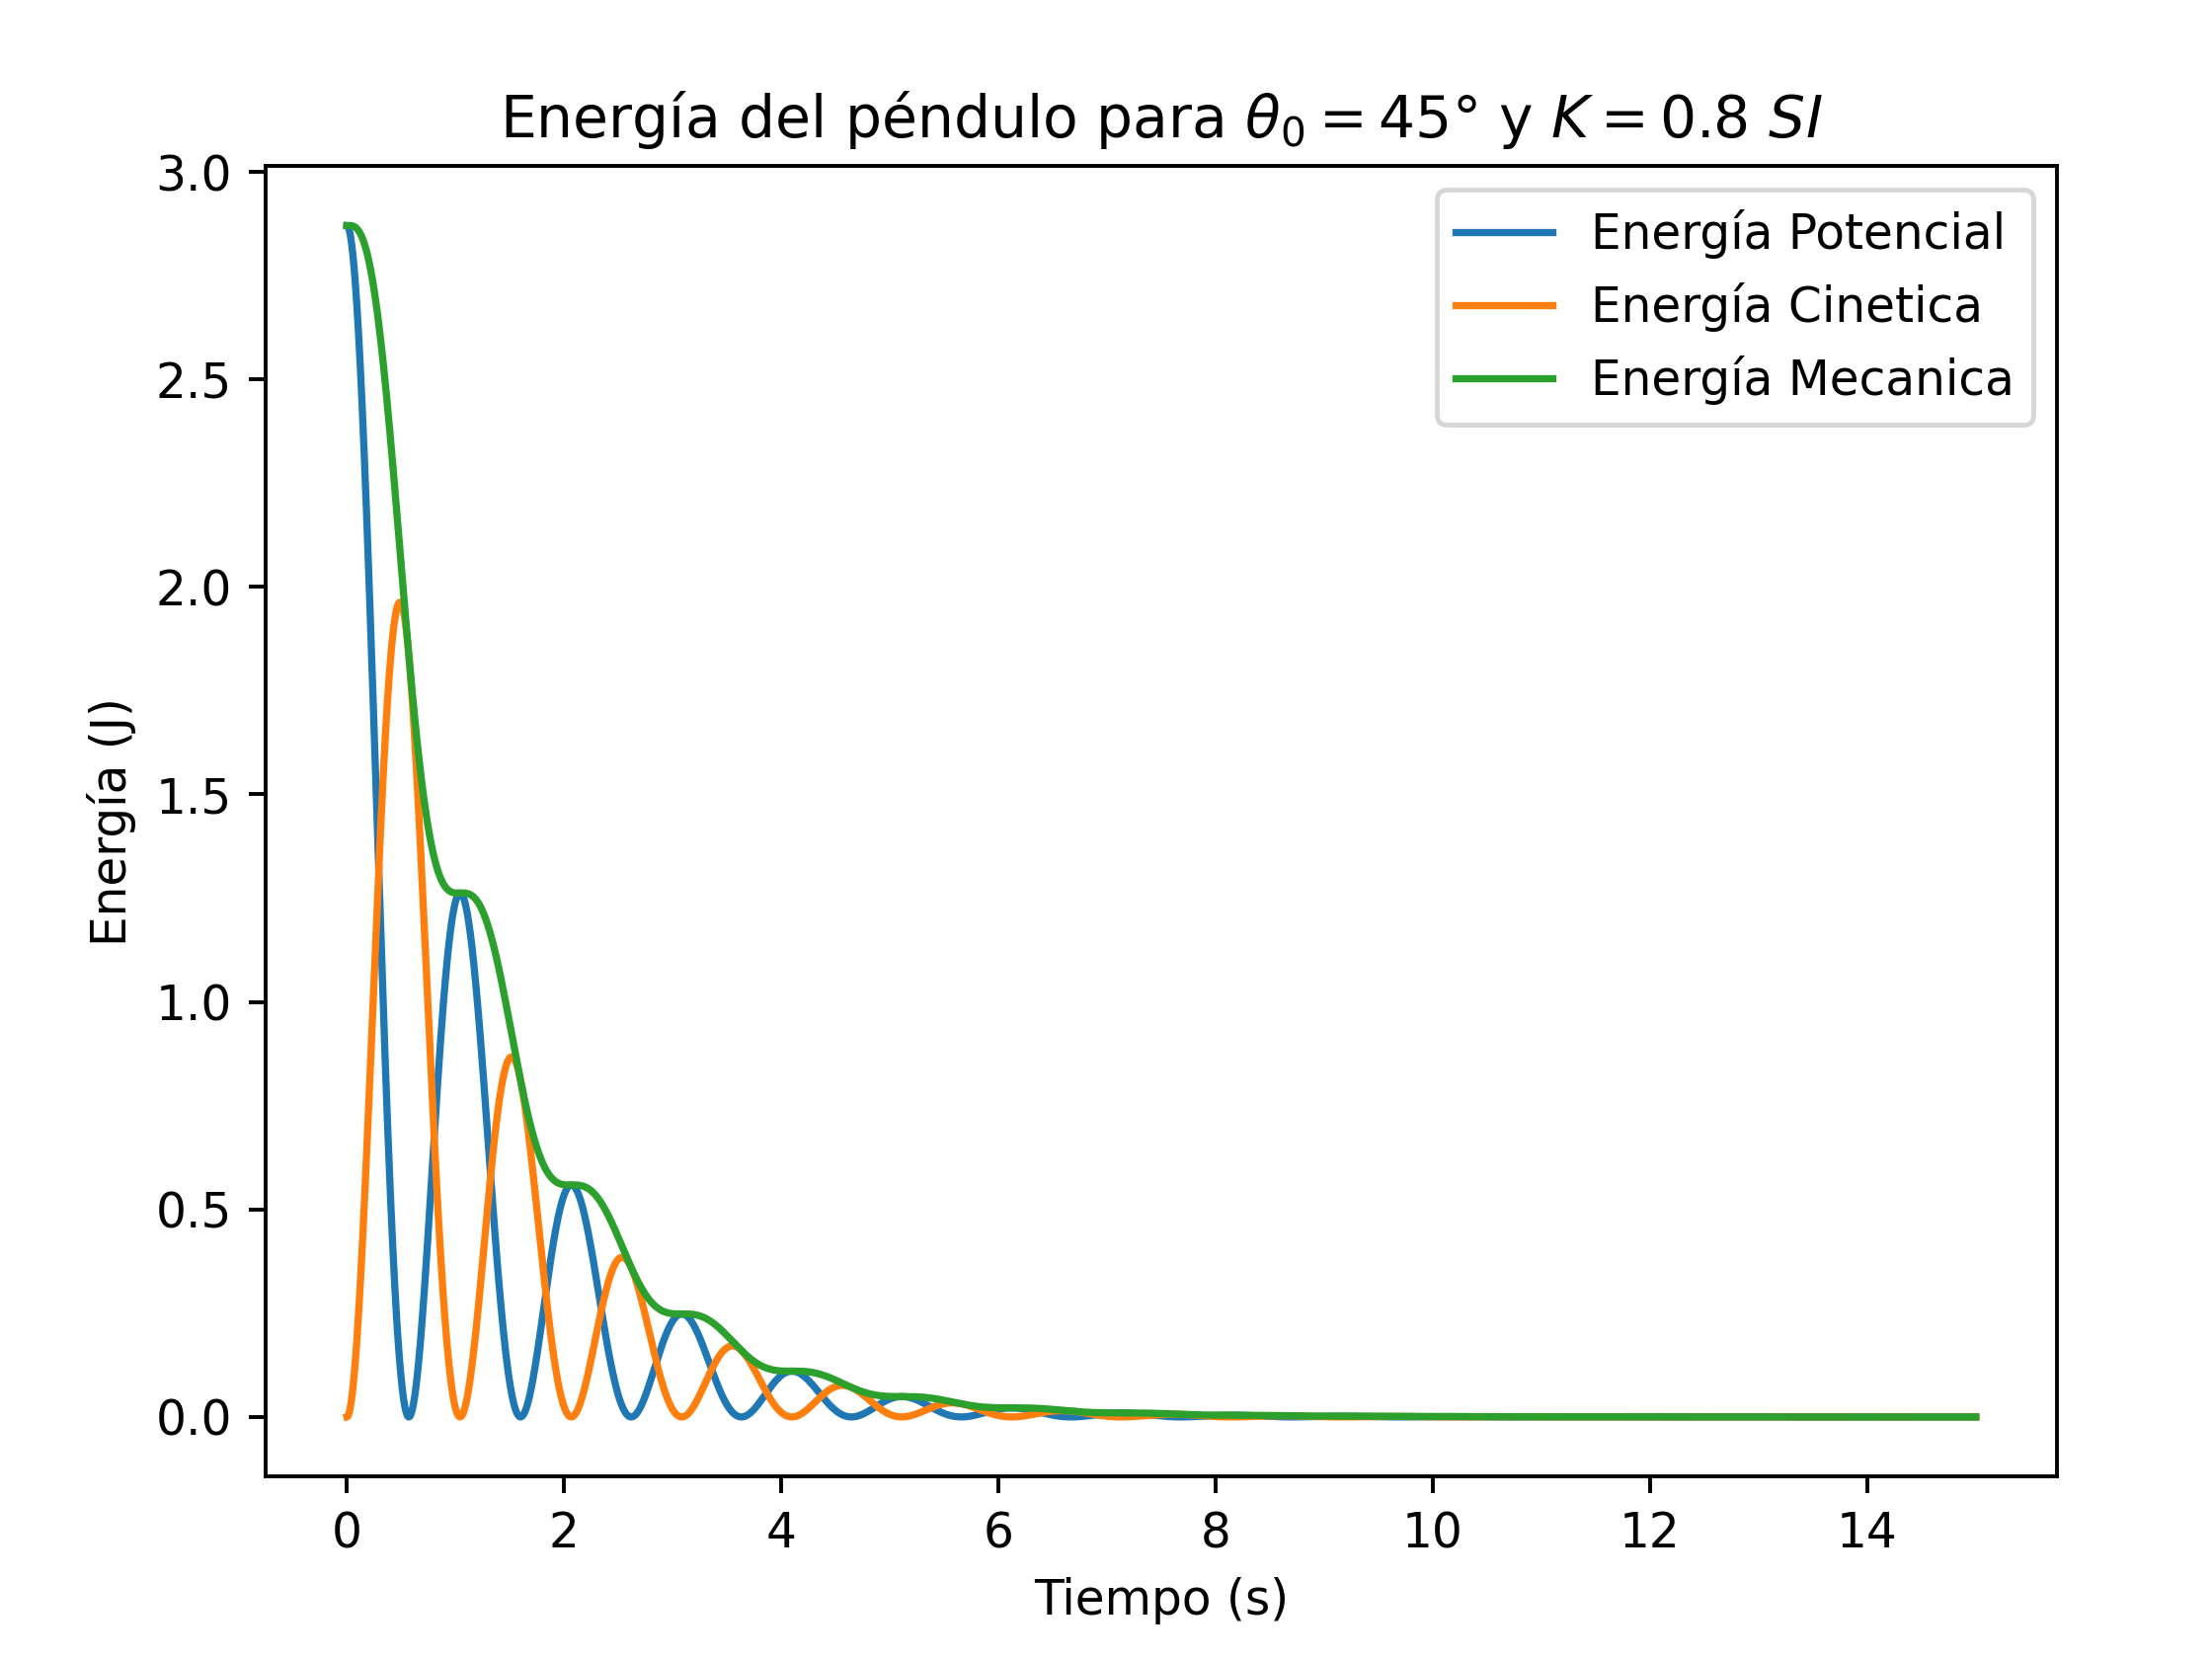
\includegraphics[width=.57\textwidth]{Fig11.png}
\end{figure}

Ahora observamos la variación de la energía para el mismo caso que con la velocidad angular y el ángulo, un péndulo soltado desde 45 grados, graficado durante 15 segundos y con varios valores de K. \\ \\La energía mecánica no se conserva, va descendiendo a lo largo del tiempo ya que estamos en un caso donde existe una fuerza disipatoria (la fuerza de rozamiento) que la va haciendo disminuir. En cada instante la energía mecánica es la suma de la potencial y la cinética. \\ \\Es interesante observar que el descenso de la energía mecánica no es una curva suave, si no que tiene una forma casi ondulatoria. Esto se debe a que la energía mecánica se disipará en mayor medida cuanto más rápido vaya el péndulo, es decir cuanto mayor sea la energía cinética. Cuando el péndulo alcanza uno de los extremos, la energía cinética será 0, y por tanto no habrá disipación. Es en estos instantes donde la energía mecánica será plana y no descenderá, lo que hace que obesrvemos estos picos en la gráfica.

\pagebreak
\hfill \break \\
\hfill \break \\
\hfill \break \\
Código que calcula la gráfica:

\lstinputlisting[language=Python, firstline=1, lastline=33]{7.py}

\pagebreak

\subsection{Cálculo del Periodo en función de K}

\begin{figure}[h]
\centering
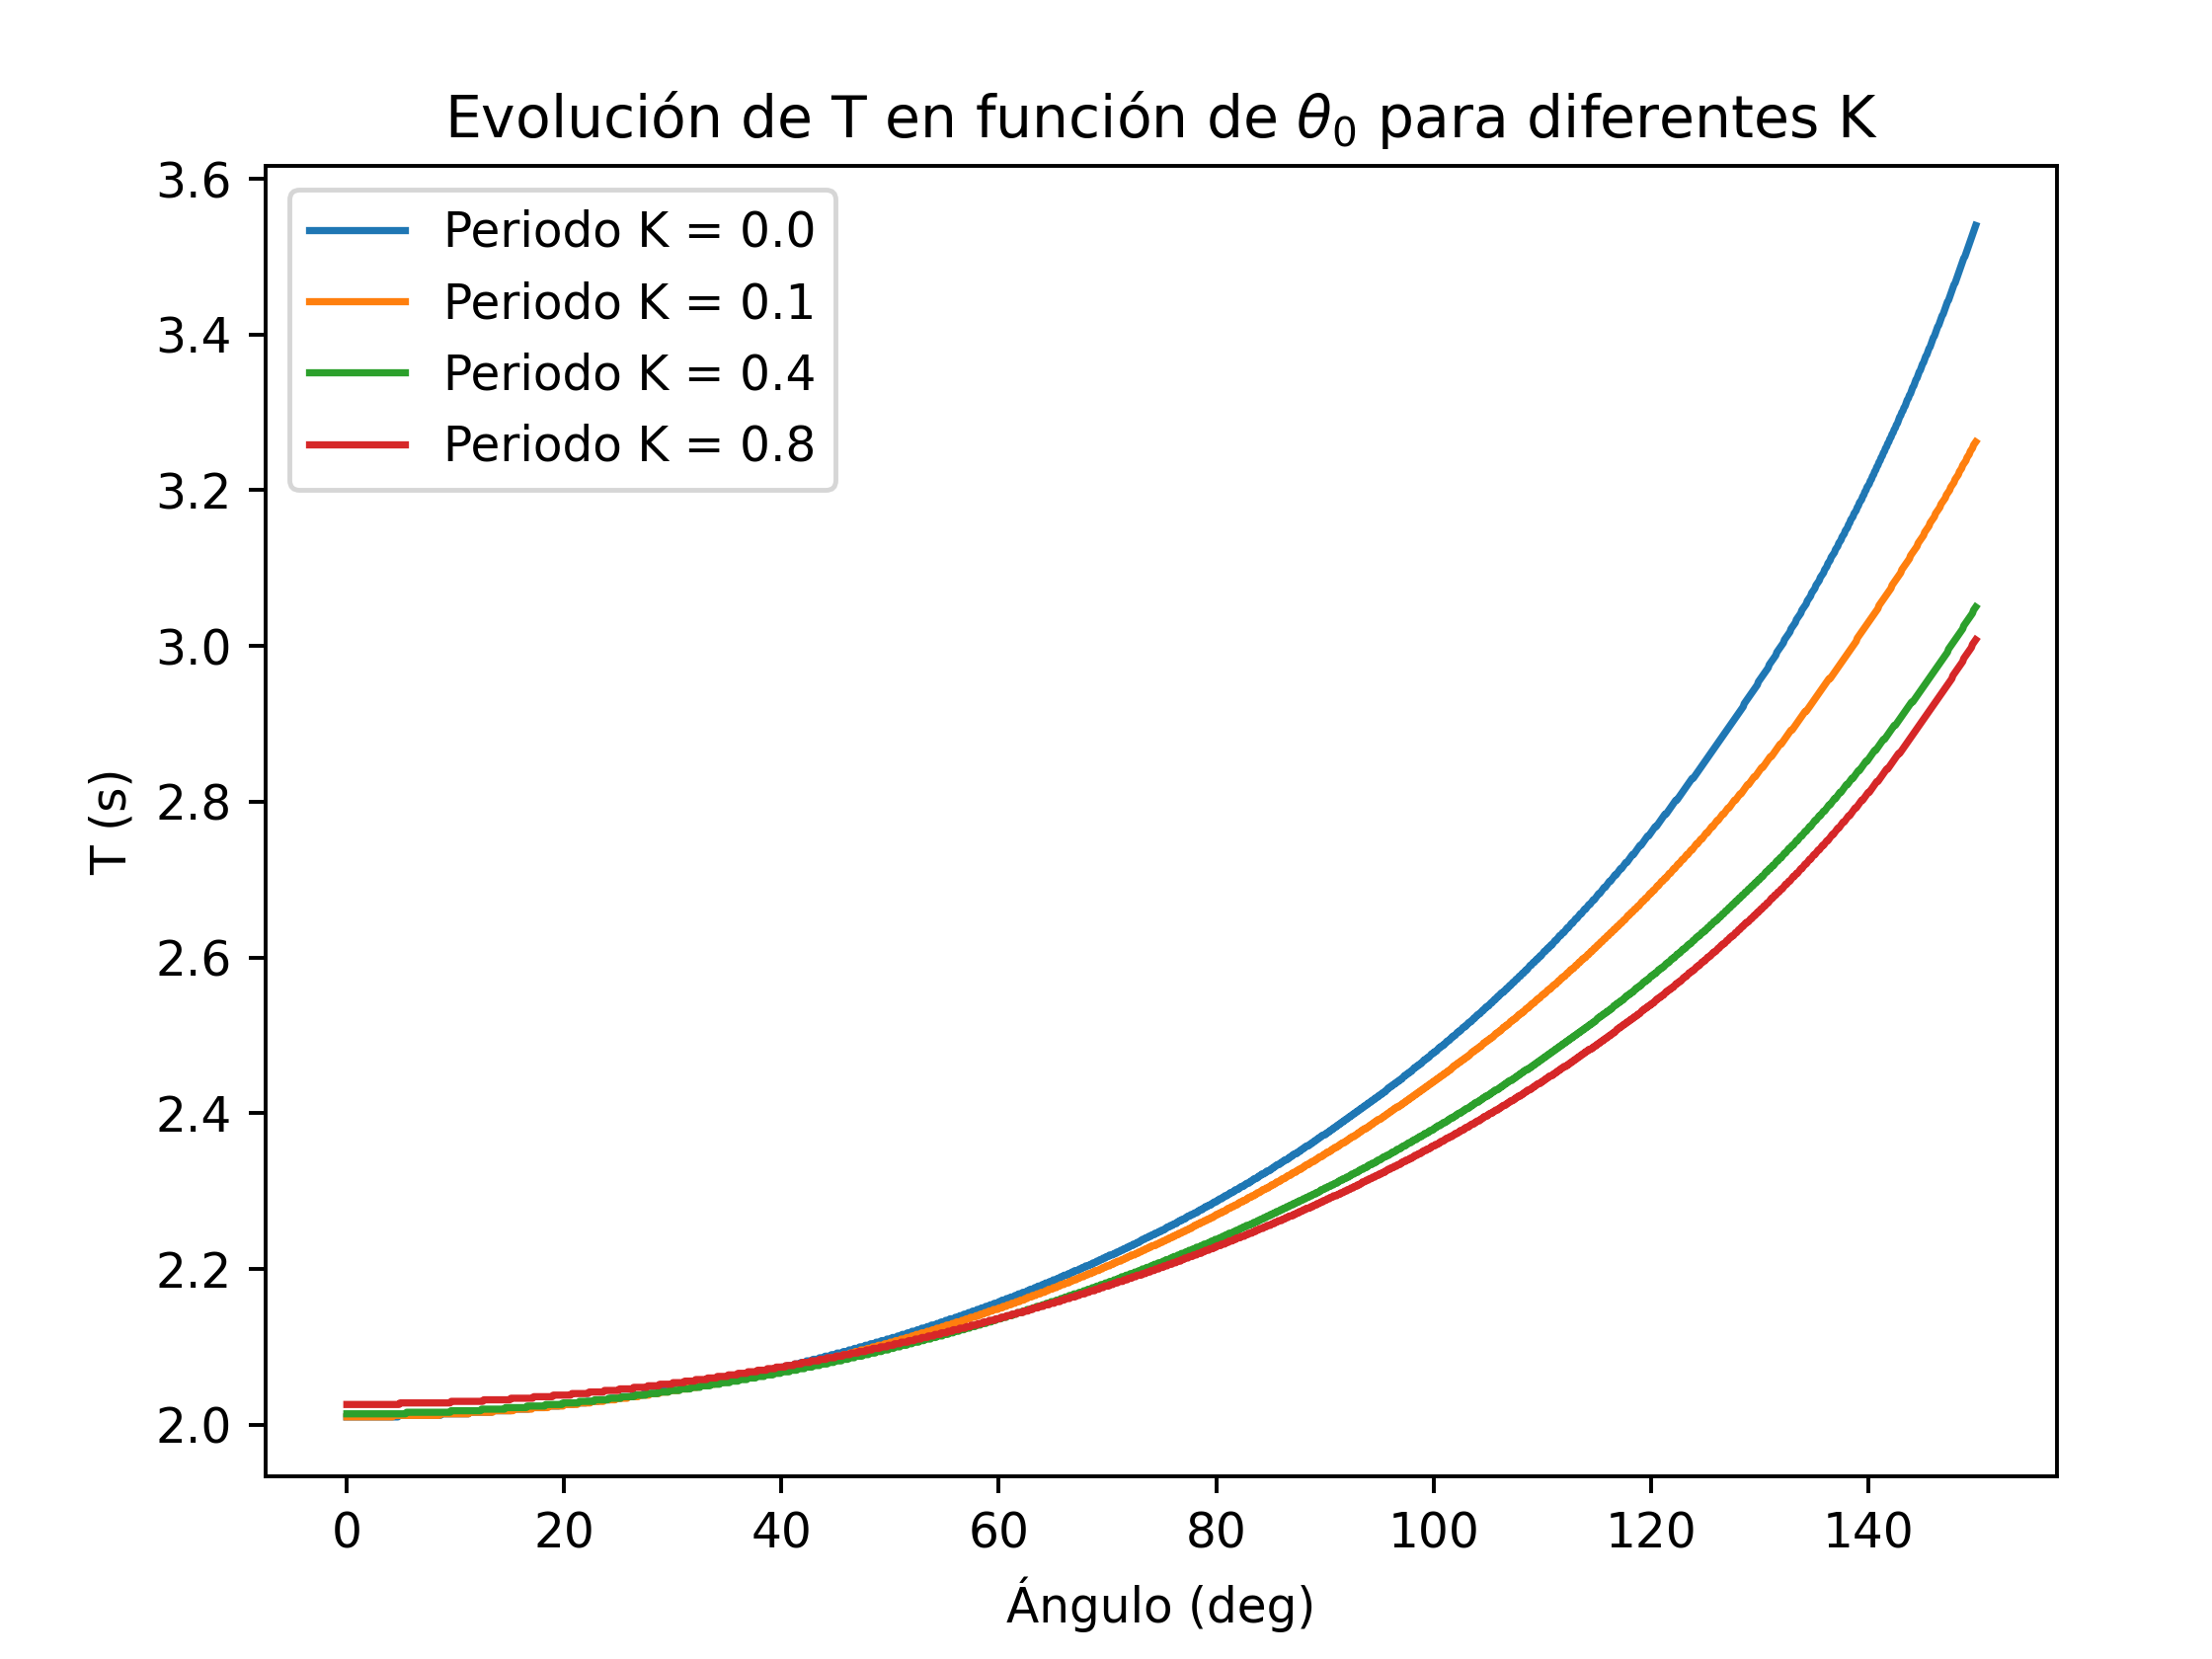
\includegraphics[width=.8\textwidth]{Fig12.png}
\end{figure}
    
\hfill \break \\
    
Por último graficaremos la evolución del periodo de la primera oscilación en el caso con rozamiento. Puesto que dependiendo del ángulo inicial desde el cual se suelte el péndulo afectará a la amplitud del ángulo, el periodo se verá afectado a su vez. Es por eso que lo graficamos en función al ángulo inicial. \\ \\ Debo mencionar que lo que se calcula para esta gráfica es en realidad el tiempo en recorrer media oscilación, que luego se multiplica por dos para aproximar el periodo total. Hago esto por motivos de eficiencia del código, que de otra forma requeriría más tiempo de ejecución. El periodo calculado diferirá con el de una oscilación completa, ya que durante la segunda parte de la oscilación seguirá habiendo rozamiento. Esto da cabida a cierto grado de error en el cálculo de la gráfica, que se agravará cuanto mayor sea la K, y mayor el rozamiento, pero que no cambiaría de forma fundamental los resultados concluidos. \\ \\ Podemos observar como para una K = 0, es decir sin rozamiento, el periodo será siempre mayor al del resto de curvas, que serán más bajas cuanto mayor sea la K, como era de esperar.
    
\pagebreak
\hfill \break \\
\hfill \break \\
Código que calcula la gráfica:
\lstinputlisting[language=Python, firstline=1, lastline=39]{8.py}
\hfill \break \\
Este código grafica la evolución del periodo en función del ángulo inicial para tantas K como le sean introducidas, si se le introduce una única K, solo graficará una, pero si se le introducen 4, graficará 4. \\ \\
El tiempo de ejecución variará drásticamente en función de cuantas curvas tenga que calcular.
% %----------------------------------------------------------------------------------------


\end{document}